
% This is the Reed College LaTeX thesis template. Most of the work 
% for the document class was done by Sam Noble (SN), as well as this
% template. Later comments etc. by Ben Salzberg (BTS). Additional
% restructuring and APA support by Jess Youngberg (JY).
% Your comments and suggestions are more than welcome; please email
% them to cus@reed.edu
%
% See http://web.reed.edu/cis/help/latex.html for help. There are a 
% great bunch of help pages there, with notes on
% getting started, bibtex, etc. Go there and read it if you're not
% already familiar with LaTeX.
%
% Any line that starts with a percent symbol is a comment. 
% They won't show up in the document, and are useful for notes 
% to yourself and explaining commands. 
% Commenting also removes a line from the document; 
% very handy for troubleshooting problems. -BTS

% As far as I know, this follows the requirements laid out in 
% the 2002-2003 Senior Handbook. Ask a librarian to check the 
% document before binding. -SN

%%
%% Preamble
%%
% \documentclass{<something>} must begin each LaTeX document
\documentclass[12pt,twoside]{reedthesis}
% Packages are extensions to the basic LaTeX functions. Whatever you
% want to typeset, there is probably a package out there for it.
% Chemistry (chemtex), screenplays, you name it.
% Check out CTAN to see: http://www.ctan.org/
%%
\usepackage{graphicx,latexsym} 
\usepackage{amssymb,amsthm,amsmath}
\usepackage{longtable,booktabs,setspace} 
\usepackage{chemarr} %% Useful for one reaction arrow, useless if you're not a chem major
\usepackage[hyphens]{url}
\usepackage{rotating}
\usepackage[numbers]{natbib}
\usepackage{color}
\usepackage{epigraph}
\usepackage{tensor}
\usepackage{bibentry}
\graphicspath{{./Figs/}} % Set graphics path
% Comment out the natbib line above and uncomment the following two lines to use the new 
% biblatex-chicago style, for Chicago A. Also make some changes at the end where the 
% bibliography is included. 
%\usepackage{biblatex-chicago}
%\bibliography{thesis}

% \usepackage{times} % other fonts are available like times, bookman, charter, palatino


%%%% REFERENCES %%%%%
\newcommand{\rf}     [1] {~\cite{#1}}
\newif\ifimagesSep
\newcommand*{\rfs}[1]{%
  \par\noindent[begin images]\\\relax
  \imagesSepfalse
  \imagesScan#1\relax\relax\relax
  [end images]\par
}
\newcommand{\imagesScan}[3]{%
  \ifx\relax#1\empty
  \else
    \ifimagesSep
      [separation]\\\relax
    \else
      \imagesSeptrue
    \fi
    [image: #1 #2 #3]\\\relax
    \expandafter\imagesScan
  \fi
}

\newcommand{\refref} [1] {ref.~\cite{#1}}
\newcommand{\refRef} [1] {Ref.~\cite{#1}}
\newcommand{\refrefs}[1] {refs.~\cite{#1}}
\newcommand{\refRefs}[1] {Refs.~\cite{#1}}
\newcommand{\refeq}  [1] {(\ref{#1})}
\newcommand{\refeqs} [2]{(\ref{#1}--\ref{#2})}
\newcommand{\reffig} [1] {figure~\ref{#1}}
\newcommand{\reffigs} [2] {figures~\ref{#1} and~\ref{#2}}
\newcommand{\refFig} [1] {Figure~\ref{#1}}
\newcommand{\refFigs} [2] {Figures~\ref{#1} and~\ref{#2}}
\newcommand{\reftab} [1] {table~\ref{#1}}
\newcommand{\refTab} [1] {Table~\ref{#1}}
\newcommand{\reftabs}[2] {tables~\ref{#1} and~\ref{#2}}
\newcommand{\refsect}[1] {Section~\ref{#1}}
\newcommand{\refsects}[2] {Sections~\ref{#1} and \ref{#2}}
\newcommand{\refSect}[1] {Sect.~\ref{#1}}
\newcommand{\refSects}[2] {Sects.~\ref{#1} and \ref{#2}}
\newcommand{\refsecttosect}[2] {Sects.~\ref{#1} to~\ref{#2}}
\newcommand{\refappe}[1] {appendix~\ref{#1}}
\newcommand{\refappes}[2] {appendices~\ref{#1} and~\ref{#2}}
\newcommand{\refAppe}[1] {Appendix~\ref{#1}}
\newcommand{\refChapter}[1]{Chapter~\ref{#1}}
\newcommand{\refChapt}[1]{Chapt.~\ref{#1}}

%%%% SYMBOLS %%%%
\newcommand{\ReN}{\ensuremath{Re}} % Reynolds number
\newcommand{\pCf}{plane Couette flow} % plane Couette flow
\newcommand{\ecs}{exact coherent structures}
\newcommand{\Ecs}{Exact coherent structures}
%%%% ABBREVIATIONS %%%%%
\newcommand{\etc}{{etc.}}       % APS
\newcommand{\etal}{{\em et al.}}    % etal in italics, APS too
\newcommand{\ie}{{i.e.}}        % APS
\newcommand{\cf}{{\em cf.\ }}     % APS
\newcommand{\eg}{{e.g.\ }}        % APS, OUP, hard space '\eg\ NextWord'

%%%%% EDITING COMMANDS %%%%%
\newcommand{\DB}[2]{$\footnotemark\footnotetext{DB #1: {\color{red}#2}}$} %date, comment
\newcommand{\DBedit}[1]{{\color{red}#1}}
\newcommand{\VGC}[2]{$\footnotemark\footnotetext{DB #1: {\color{blue}#2}}$} %date, comment
\newcommand{\VGedit}[1]{{\color{blue}#1}}


%%%% SUPER USEFUL COMMANDS THAT I'M USED TO HAVING%%%%%
\let\Oldfrac\frac
\renewcommand{\frac}[2]{\dfrac{#1}{#2}}

\let\Oldsin\sin
\renewcommand{\sin}[1]{\Oldsin{\left ( #1  \right ) }}

\let\Oldcos\cos
\renewcommand{\cos}[1]{\Oldcos{\left ( #1  \right ) }}

\newcommand{\abs}[1]{\left | #1 \right |}
\newcommand{\sqfrac}[2]{\sqrt{\frac{#1}{#2}}}
\newcommand{\paren}[1]{\left ( #1 \right )}
\newcommand{\sbrac}[1]{\left [ #1 \right ]}
\newcommand{\scprod}[3]{\left < #1,#2 \right >_{#3}}

\let\Oldint\int
\renewcommand{\int}[4]{\Oldint_{#1}^{#2} #3 \hspace{2mm}#4}
\let\Oldsum\sum
\renewcommand{\sum}[3]{\Oldsum\limits_{#1}^{#2} #3}


\newcommand{\pder}[3]{\ifnum#1=1
							\dfrac{\partial#2}{\partial#3}
					   \else
					   \ifnum#1>1\dfrac{\partial^{#1}#2}{\partial#3^{#1}} \fi \fi }
\newcommand{\der}[3]{\ifnum#1=1
							\dfrac{\text{d}#2}{\text{d}#3}
					   \else
					   \ifnum#1>1\dfrac{\text{d}^{#1}#2}{\text{d}#3^{#1}} \fi \fi }
\newcommand{\Vector}[1]{\mathbf{#1}}
\newcommand{\Tensor}[1]{\mathcal{#1}}
\newcommand{\function}[2]{#1\!\paren{#2}}

\newcommand{\Div}[1]{\nabla\cdot#1}
\newcommand{\Grad}[1]{\nabla\,#1}
\newcommand{\equationref}[1]{Equation~\ref{#1}}
\newcommand{\figureref}[1]{Figure~\ref{#1}} % Load thesis specific macros

\title{Exact Coherent Structures with Broken Symmetry in Plane Couette Flow}
\author{Varchas Gopalaswamy}
% The month and year that you submit your FINAL draft TO THE LIBRARY (May or December)
\date{\today}
\division{Mathematics and Natural Sciences}
\advisor{Daniel Borrero}
%If you have two advisors for some reason, you can use the following
%\altadvisor{Your Other Advisor}
%%% Remember to use the correct department!
\department{Physics}
% if you're writing a thesis in an interdisciplinary major,
% uncomment the line below and change the text as appropriate.
% check the Senior Handbook if unsure.
%\thedivisionof{The Established Interdisciplinary Committee for}
% if you want the approval page to say "Approved for the Committee",
% uncomment the next line
%\approvedforthe{Committee}

\setlength{\parskip}{0pt}
%%
%% End Preamble
%%
%% The fun begins:
\begin{document}

  \maketitle
  \frontmatter % this stuff will be roman-numbered
  \pagestyle{empty} % this removes page numbers from the frontmatter

% Acknowledgements (Acceptable American spelling) are optional
% So are Acknowledgments (proper English spelling)
	% Acknowledgements (Acceptable American spelling) are optional
% So are Acknowledgments (proper English spelling)
    \chapter*{Acknowledgments}
	\epigraph{Some people are of the opinion that acknowledgments ought to be concise, relevant to the thesis, and devoid of sappy sentiment. They are probably right, but they aren't the ones writing this.}{Varchas Gopalaswamy}

This thesis wouldn't have existed without my thesis advisor, Daniel Borrero. Thank you, Daniel, for suggesting an awesome thesis topic, for motivating me, for spending a ton of time correcting more terrible thesis drafts than any human should have to, for introducing me to dynamical systems theory, and for all the grad school help. Good luck with setting up the Taylor-Couette system.\\

I would also like to thank John Gibson from the University of New Hampshire for making this thesis even remotely feasible by writing {\tt Channelflow}, and for taking the time to correspond with me via email and Hangout. Your advice has been invaluable. \\
 
By definition, this thesis wouldn't have existed were I not a physics major, so I'd like to thank the department as a whole for being the greatest department at Reed. Thank you, Lucas, for being an extremely supportive academic advisor and for a  challenging junior year. Thank you, Joel, for introducing me to the world of scientific computation, for running physics softball, and for your help with this thesis. Thank you, Darrell, for reminding me why quantum mechanics is awesome. Thank you, Johnny, for all the help with the grad school process. Thanks also to the physics seniors -- shoutout to Julia and Neal for their tenure as the Pub Czars, Taras for his tenure as the Cookie Czar, Dan for putting up with the frantic late night calls for help, and Newton for being a rad office buddy.  I will be proud to say that I was once a part of this group. You guys have made my time here special. \\

To Amma and Appa -- Thank you for all your love and support throughout all these years, and always being understanding and there for me when I have the occasional mental breakdown. Also, thanks for going ``Yes, let's send Varchas to this college we've literally never heard anything about, this sounds like a great idea." I hope you feel that you've made the right decision. 

Dear Medha: Thank you for allowing me to lecture at you about stuff you may or may not actually be interested in, for enabling me in some truly horrendous jokes, for doing all the housework whenever I would come back for vacation, and generally being an awesome sister. \\

To all my friends -- Thank you for making Reed the best of times, and for supporting me through the worst of times. Words cannot express how much I will miss you all.\footnote{Yes Matt, even you.}






% The preface is optional
% To remove it, comment it out or delete it.
%	% The preface is optional
% To remove it, comment it out or delete it.
    \chapter*{Preface}
	This is an example of a thesis setup to use the reed thesis document class.

\tableofcontents

% if you want a list of tables, optional
%  \listoftables
% if you want a list of figures, also optional
  \listoffigures
		
% The abstract is not required if you're writing a creative thesis (but aren't they all?)
% If your abstract is longer than a page, there may be a formatting issue.
	%% The abstract is not required if you're writing a creative thesis (but aren't they all?)
% If your abstract is longer than a page, there may be a formatting issue.
    \chapter*{Abstract}
	\Ecs are an exciting and potentially revolutionary method of understanding turbulent dynamics and transition. In \pCf, the inherent symmetries naturally lead to symmetric \ecs, which are computationally easier to find. However, turbulence itself is a fundamentally asymmetric phenomenon, and may be better described by symmetry broken \ecs. In this thesis, we find four new periodic orbits -- P85 and P60m which have unbroken symmetry and P32 and P8, which have partially broken symmetry, using the computational fluid dynamics library {\tt Channelflow}. Comparison of the projections of these periodic orbits in the dissipation-energy input plane with randomly seeded turbulent trajectories reveals that P32, P60 and P85 lie in the turbulent region, while P8 lies very far away from the turbulent region. Nevertheless, we focus on P8 so as to best utilize limited computational resources. Parametric continuation in the spanwise periodic cell length $L_z$ suggests that P8 undergoes two bifurcations. This is verified by analysis of various properties of P8 in the dissipation-energy input plane, as well as an observation of a change of stability of eigenvectors that are consistent with the bifurcation.   
	%	\chapter*{Dedication}
	To Perfect Woodbridge \\
	\emph{sic transit gloria mundi}

  \mainmatter % here the regular arabic numbering starts
  \pagestyle{fancyplain} % turns page numbering back on

% Double spacing: if you want to double space, or one and a half 
% space, uncomment one of the following lines. You can go back to 
% single spacing with the \singlespacing command.
% \onehalfspacing
% \doublespacing

	%The \introduction command is provided as a convenience.
%if you want special chapter formatting, you'll probably want to avoid using it altogether
		\setcounter{secnumdepth}{0}
\chapter*{Introduction}
    \addcontentsline{toc}{chapter}{Introduction}
		\chaptermark{Introduction}
		\markboth{Introduction}{Introduction}

% The three lines above are to make sure that the headers are right, that the intro gets included in the table of contents, and that it doesn't get numbered 1 so that chapter one is 1.
\epigraph{ I am an old man now, and when I die and go to heaven, there are two matters on which I hope for enlightenment. One is quantum electrodynamics, and the other is the turbulent motion of fluids. And about the former, I am optimistic. }{Horace Lamb, 1932}
	
Although much work has been done in understanding turbulence since Lamb's time, the twin problems of understanding the nature of the transition to turbulence and predicting the fine structure of turbulent flows remain unsolved to this day, having vexed scientists and engineers in much the same way a plucky band of Gauls did for Caesar. Understanding turbulence is vitally important, since turbulent flows appear in man-made scenarios such as the flow around ships or aircraft, as well as in natural scenarios like the atmosphere of Jupiter and the flow of blood in the heart. The degree to which a flow is turbulent is characterized by its {\bf Reynolds number} \ReN, a dimensionless parameter that encodes the relative importance of inertial and viscous forces. At small \ReN, the {\bf viscosity} of a fluid (which is analogous to fluid friction) dominates, and smooths out velocity gradients in the flow, resulting in well-ordered, {\bf laminar} flow. At large \ReN, kinetic energy is dissipated at a lower rate, allowing for the existence of increasingly complex flow structures such as eddies or vortices (\refFig{fig:cylinderWake}). These structures, which are typical of {\bf turbulence}, display large spatiotemporal variations and structure at a variety of spatial and temporal scales.
\begin{figure}[h]
\centerline{
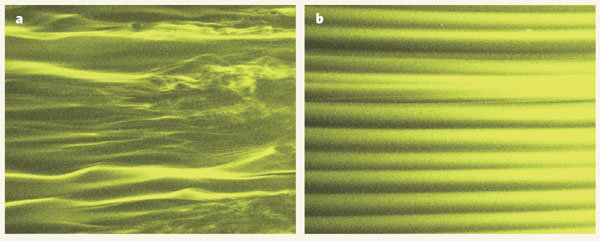
\includegraphics[width=\textwidth]{Figs/laminarTurbulent}}
\caption[Streamlines on two surfaces of differing smoothness showcase the difference between laminar and turbulent flows.]{Streamlines on two surfaces of differing smoothness showcase the difference between laminar and turbulent flows. (a) In turbulent flow across an extremely smooth surface, streamlines break up into chaotic eddies and swirls, while in (b), the laminar flow across a rough surface preserves the streamlines. Reproduced from K.S. Choi, ``Fluid Dynamics: The rough with the smooth", \emph{Nature},  vol. 440, no, 7085, pp. 754-754, 2006\rf{Choi2006}.}\label{fig:cylinderWake}
\end{figure}
\begin{figure}[h!]
\centerline{
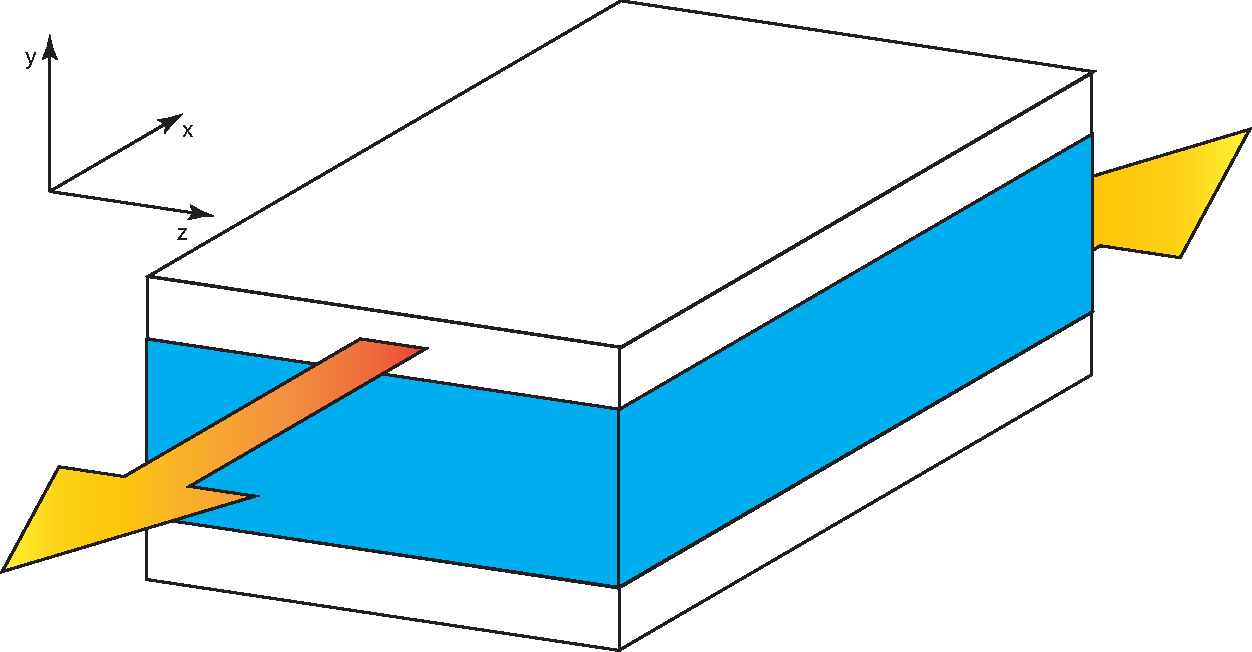
\includegraphics[scale=0.4]{Figs/planeCouetteDiagram}}
\caption[A schematic of the plane Couette geometry.]{A schematic of the plane Couette geometry. The upper and lower plates (white) extend infinitely in the plane, as does the fluid (blue) filling the gap between them. The upper and lower plates move with some constant velocity, and apply shear stresses to the fluid, resulting in fluid motion. While in general the plates can move in any direction, there is always a reference frame in which the plates move with equal but opposite velocity and it is convenient to work in this reference frame. According to convention, the $x$ axis is aligned along the plate velocity and is referred to as the {\bf streamwise} direction. The $y$-axis is aligned perpendicular to the plates and is referred to as the {\bf wall-normal} direction. The $z$-axis is normal to both axes and is referred to as the {\bf spanwise} direction.}\label{fig:planeCouette}
\end{figure}

\section{Plane Couette Flow} 

Since viscosity is a dissipative force, a viscous fluid that has no energy input will eventually come to rest as its kinetic energy is dissipated into thermal energy. Therefore, sustaining turbulence requires continuous energy input. In the case of the flow between two infinite parallel plates (\refFig{fig:planeCouette}), which is known as \pCf\ and is the focus of this thesis, this is provided by the wall shear. The geometry of the plane Couette system is extremely simple, with a geometrical parameter $h$, the half-distance between the parallel plates, and a kinematic parameter $V$, the constant velocity of the upper plate. This gives the Reynolds number as 
\begin{equation}
\ReN = \frac{hV}{\nu},
\end{equation}
where $\nu$ is the kinematic viscosity of the fluid. When \ReN~is very small, only the laminar flow state is stable. In the case of \pCf\ this corresponds to a linear velocity profile, shown in \refFig{fig:planeCouetteBulk}. As \ReN~increases, experiments\rf{Daviaud1992} have demonstrated the existence of long-lived turbulent flows, despite the fact that linear stability analysis predicts that the laminar state should remain stable.
\begin{figure}
\centerline{
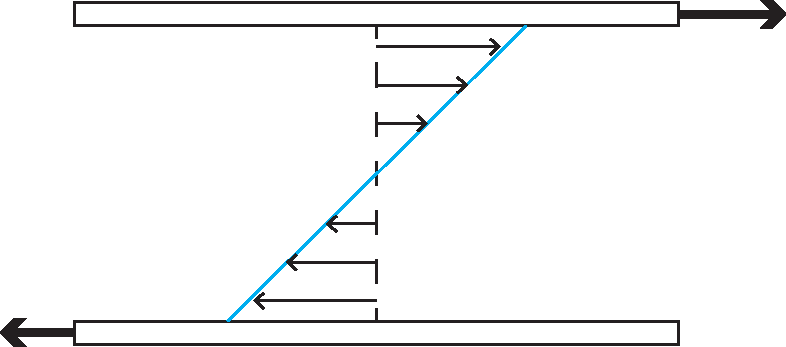
\includegraphics[scale=0.6]{Figs/planeCouetteMeanFlow}}
\caption[A cross-sectional representation of \pCf, with the linear, laminar velocity profile shown.]{A cross-sectional representation of \pCf, with the linear, laminar velocity profile shown. By symmetry, the laminar profile must be the same everywhere. At the top and bottom, where the fluid meets the walls, no-slip boundary conditions require that the wall-tangent velocity equal the boundary velocity.}\label{fig:planeCouetteBulk}
\end{figure}

\section{Tackling Turbulence} 

The traditional approach for the analysis of turbulent flow is the statistical approach initially developed by Reynolds, Prandtl, von Karman, Kolmogorov and others\rf{Pope2000}. At the core of the statistical approach to turbulence is the assumption that turbulent flow states can be expressed as random perturbations around some mean flow. At high \ReN, where direct numerical simulation (DNS) of the flow is computationally infeasible,\footnote{In essence, this is due to the fact that the minimum computational resolution required for DNS scales as $\ReN^{2.25}$ in 3D. As a result, the numerical resolution required to resolve even moderate \ReN\ flows is huge.}  the statistical approach is invaluable. However, at low-to-moderate \ReN, these models can become less accurate\rf{Pope2000}. Even ignoring the moderate \ReN\ behavior of the statistical models, a fundamental problem with the statistical approach is that it discards much of the dynamical information about turbulence. Some statistical methods like Reynolds Averaged Navier-Stokes choose to time-average the Navier-Stokes equations, while others like Large Eddy Simulations model all small length scale behavior, resolving only large length scales. For this reason, it seems likely that while statistical methods will remain fundamental to applied computational fluid dynamics (CFD), especially in engineering practice, they cannot truly provide an answer to the turbulence problem. \\

An alternate approach was proposed by Eberhard Hopf in 1948\rf{Hopf1948}. Hopf suggested that solutions to the Navier-Stokes equations might be thought of as trajectories in an infinite dimensional state space in which each point corresponded to a possible velocity field. To better understand what this would mean, consider the mean velocity field of some infinitesimal volume of fluid, pictured in \refFig{fig:VectorSpace}. In order to describe the velocity at a point in the fluid, three numbers are required (each of which can take any real value), so this vector lives in a three dimensional vector space. Now any finite fluid volume will have an infinite number of points at which the velocity field has to be specified, so we would need an infinite set of numbers to describe the full velocity field. An object that would keep track of all these numbers would form an infinite dimensional vector $\Vector{v} = \{v_{i,1},v_{i,2},v_{i,3}...\},~i \in \mathbb{R}$, so that any flow state would be represented by a unique vector in this infinite dimensional vector space, which is known as the {\bf state space}. 


\begin{figure}
\centerline{
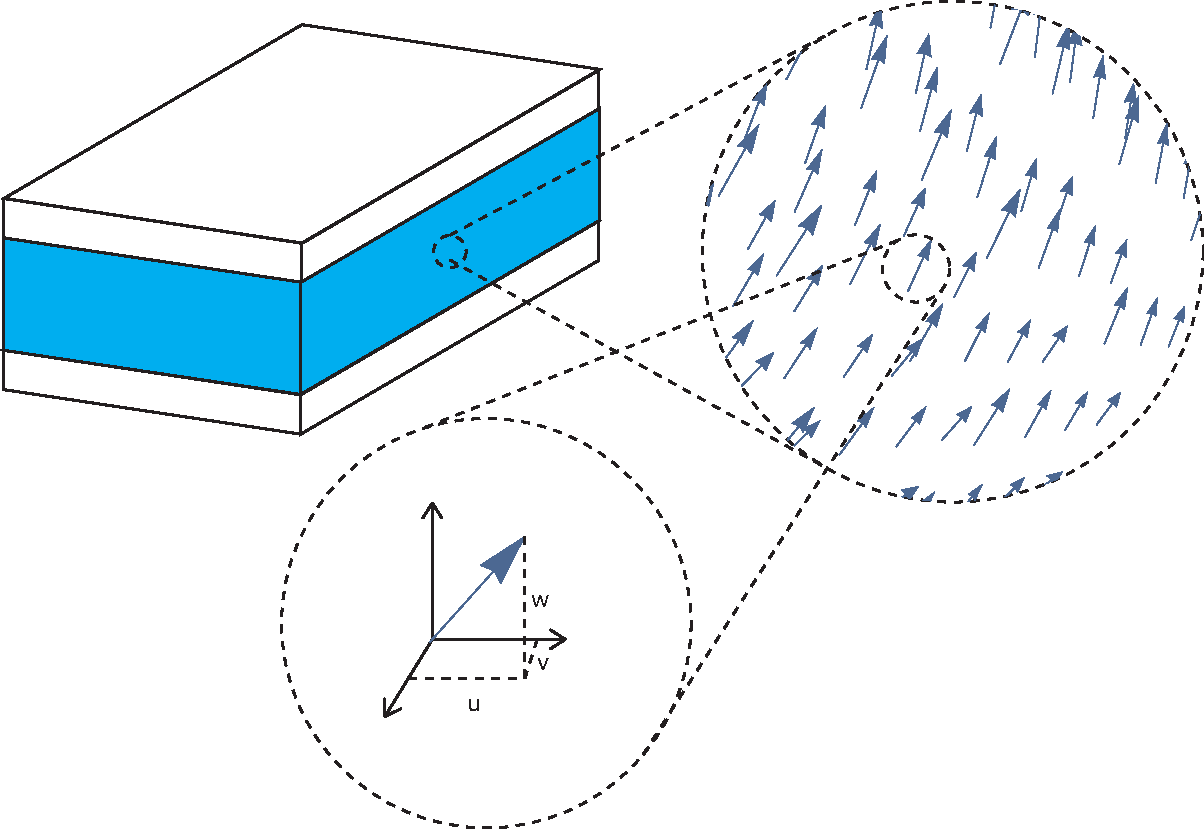
\includegraphics[scale=0.6]{Figs/VectorSpace}}
\caption{At each point in the fluid volume, the velocity field has a value that is described by three numbers, thus requiring three dimensions to track over time.}\label{fig:VectorSpace}
\end{figure}


Luckily, every point in the space does not necessarily correspond to a solution of the Navier-Stokes equation; for a given finite \ReN, for instance, the gradient of the velocity field cannot be too large since it would be smoothed out by viscosity. Hopf thus conjectured that physical trajectories corresponding to solutions to the Navier-Stokes equation would lie on some finite-dimensional manifold (known as the {\bf inertial manifold}) embedded within this infinite dimensional space. The restriction of dynamics from the infinite dimensional space to a finite dimensional inertial manifold due to the variation of a control parameter\footnote{The control parameter of a dynamical system is a number that is time-independent, and typically dictates the behavior of the system in some way. For instance, in the dimensionless simple harmonic oscillator, $\ddot{x} + 2\zeta \dot{x} + x = 0$, the control parameter is the dimensionless number $\zeta$, whose value determines whether the system is undamped, underdamped, over damped or critically damped.} has been rigorously proven under certain conditions\rf{Foias1988}. For the Navier-Stokes equation, the inertial manifold's control parameter is \ReN, and physical intuition suggests that its structure should also have \ReN~dependence, since at very low \ReN, the only physical solution is the laminar state which corresponds to a point in the state space. As \ReN\ increases, more complex flows become physically permissible, so the inertial manifold grows from a point of dimension 0 into a more complex, higher dimensional manifold. Hopf proposed that turbulence in this view was simply a trajectory that would travel across wide distances on the inertial manifold. \\


\begin{figure}[h]
\centerline{
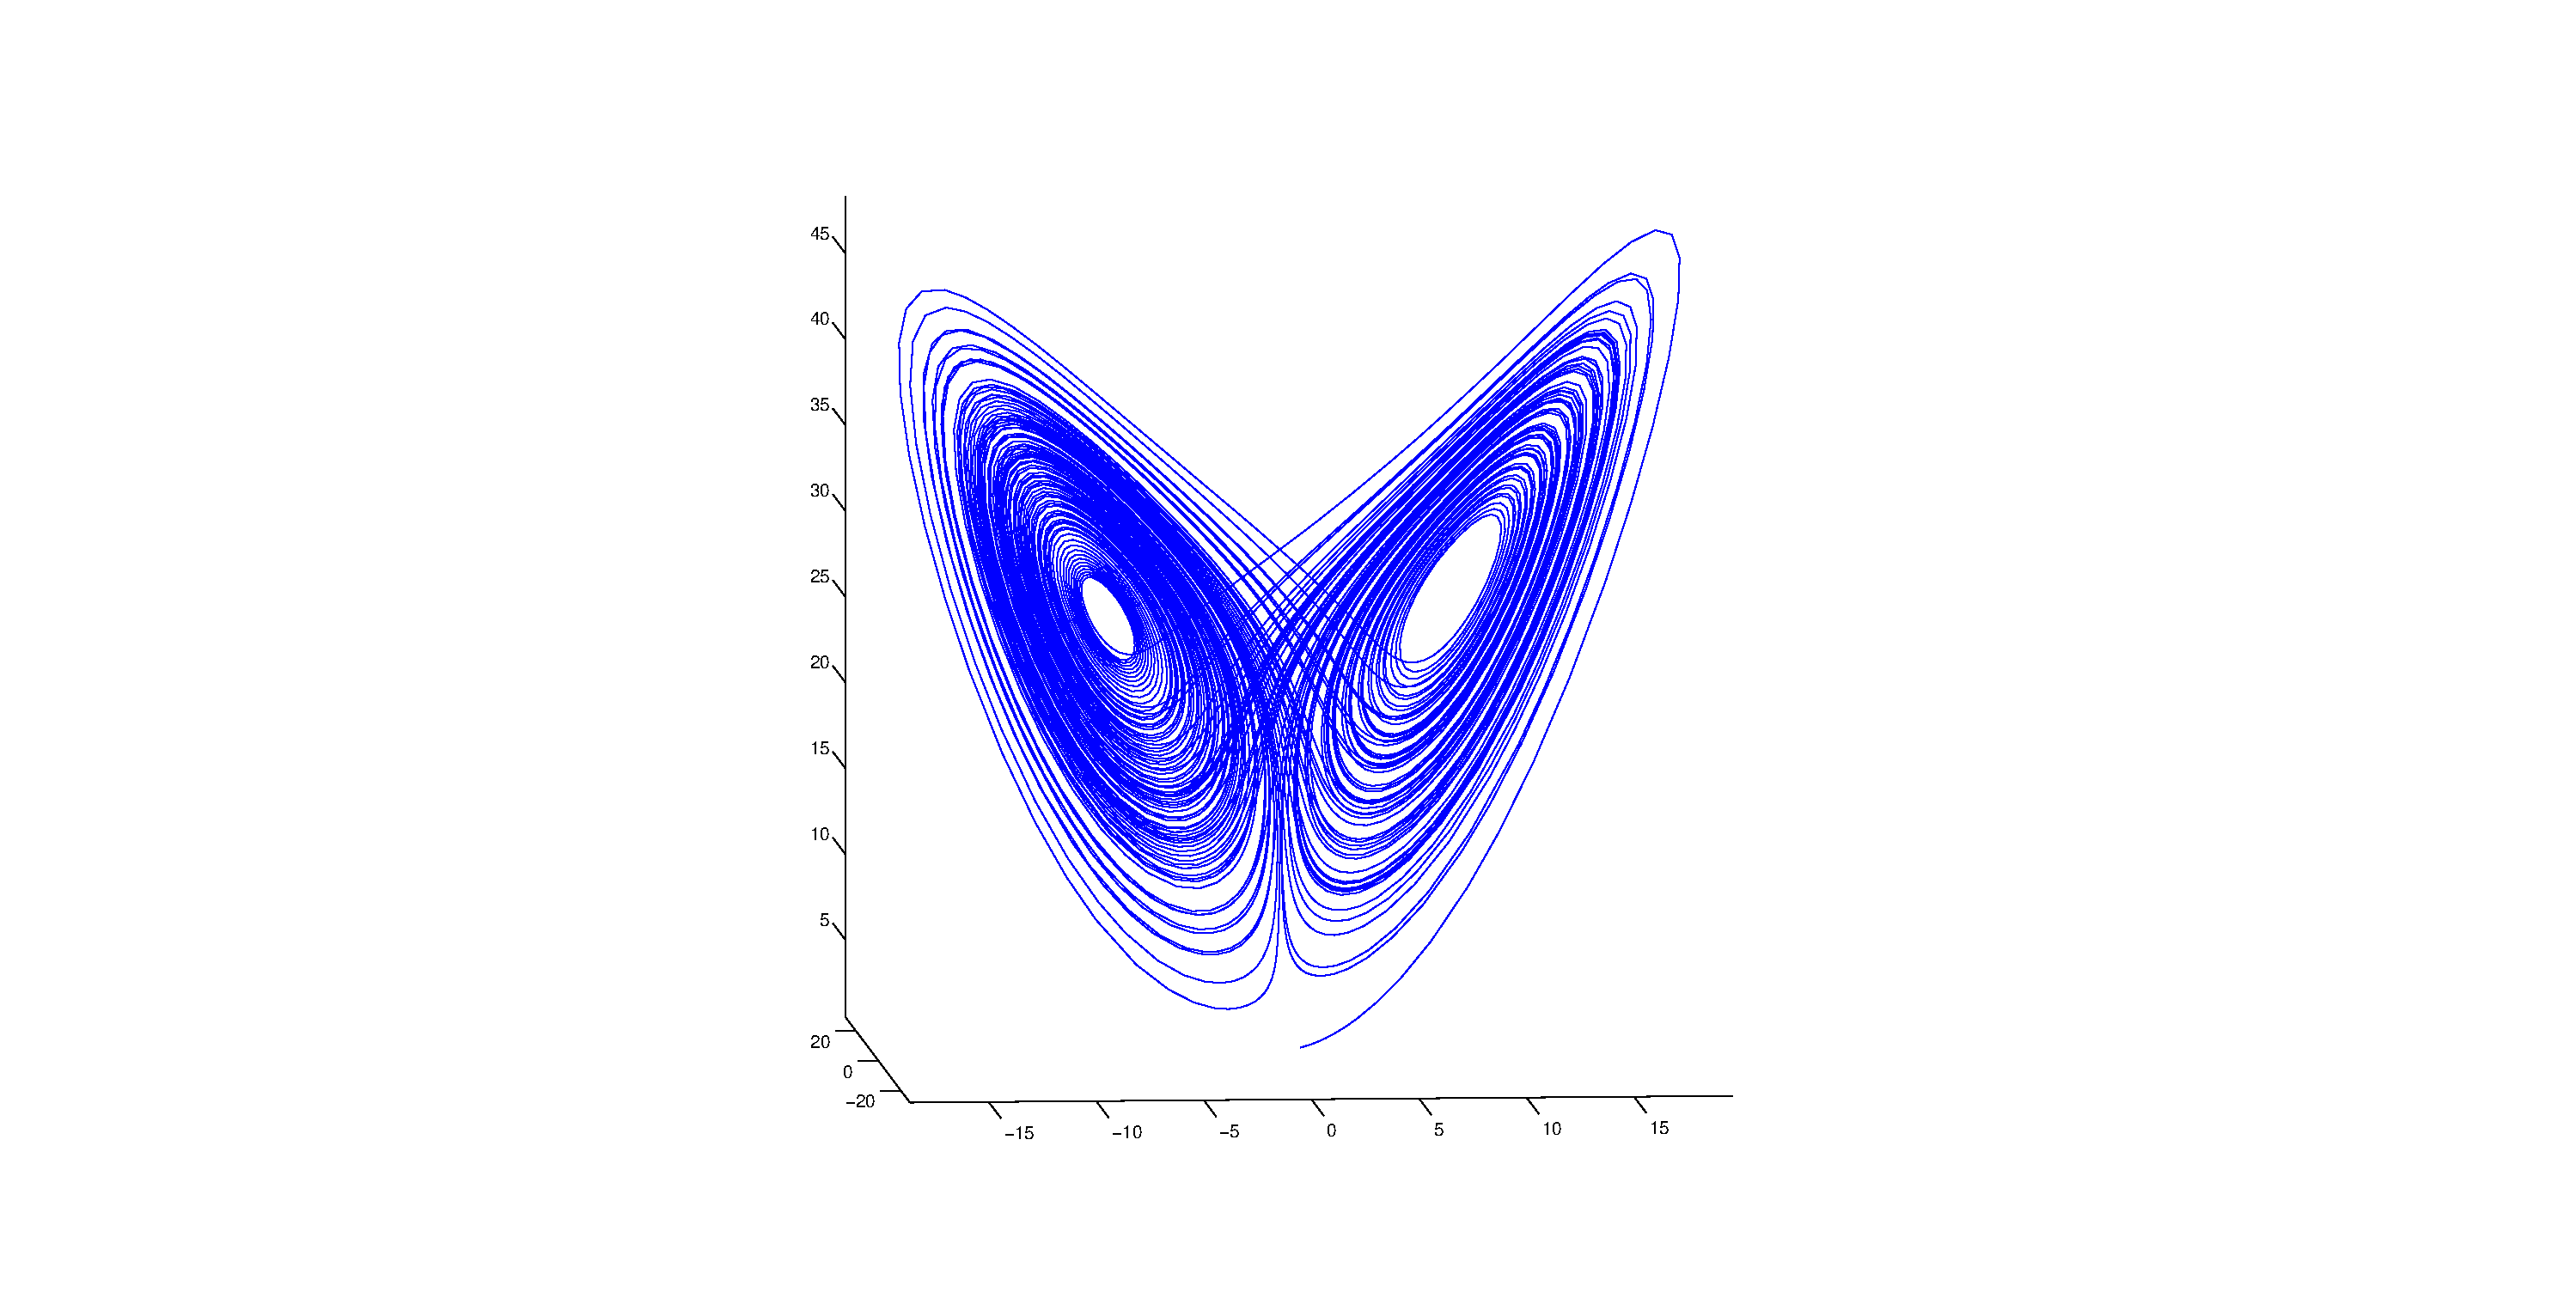
\includegraphics[scale=0.5	]{Figs/LorenzAttractor}}
\caption[A plot of a trajectory for the Lorenz system.]{A plot of a trajectory for the Lorenz system. The Lorenz system is an excellent example of a system in which the dynamics collapse onto an inertial manifold - in this case, the dynamics exist on a manifold of fractal dimension 2.06\rf{Grassberger2004}, even though the state space is in three dimensions. }\label{fig:LorenzAttractor}
\end{figure}

Unfortunately for Hopf, the computer power necessary to pursue this line of work was not available in 1948, leading him to comment in frustration that ``“the great mathematical difficulties of these important problems are well
known and at present the way to a successful attack on them seems hopelessly
barred"\rf{Hopf1948}. It would take until 1963 and the derivation of the Lorenz system (\refFig{fig:LorenzAttractor}) for the first numerical state-space analysis of turbulence\rf{Lorenz1963}, albeit for a highly truncated version of Navier-Stokes, designed to investigate Rayleigh-Bernard convection.\footnote{Interestingly, Lorenz truncated Navier-Stoke via a Galerkin approximation, which is what the simulation library {\tt Channelflow} which features heavily in this thesis also does, though it allows for many more Fourier modes than Lorenz did.} There have also been a number of efforts to explore the structure of invariant manifolds in moderate \ReN\ turbulence Navier-Stokes, such as Proper Orthogonal Decomposition\rf{Aubry1988} and the `self-sustaining process theory'\rf{Dauchot2000}, which while fruitful, are nevertheless models of turbulent flow, and not an exact analysis of the Navier-Stokes equations.\\


\begin{figure}[h]
\centerline{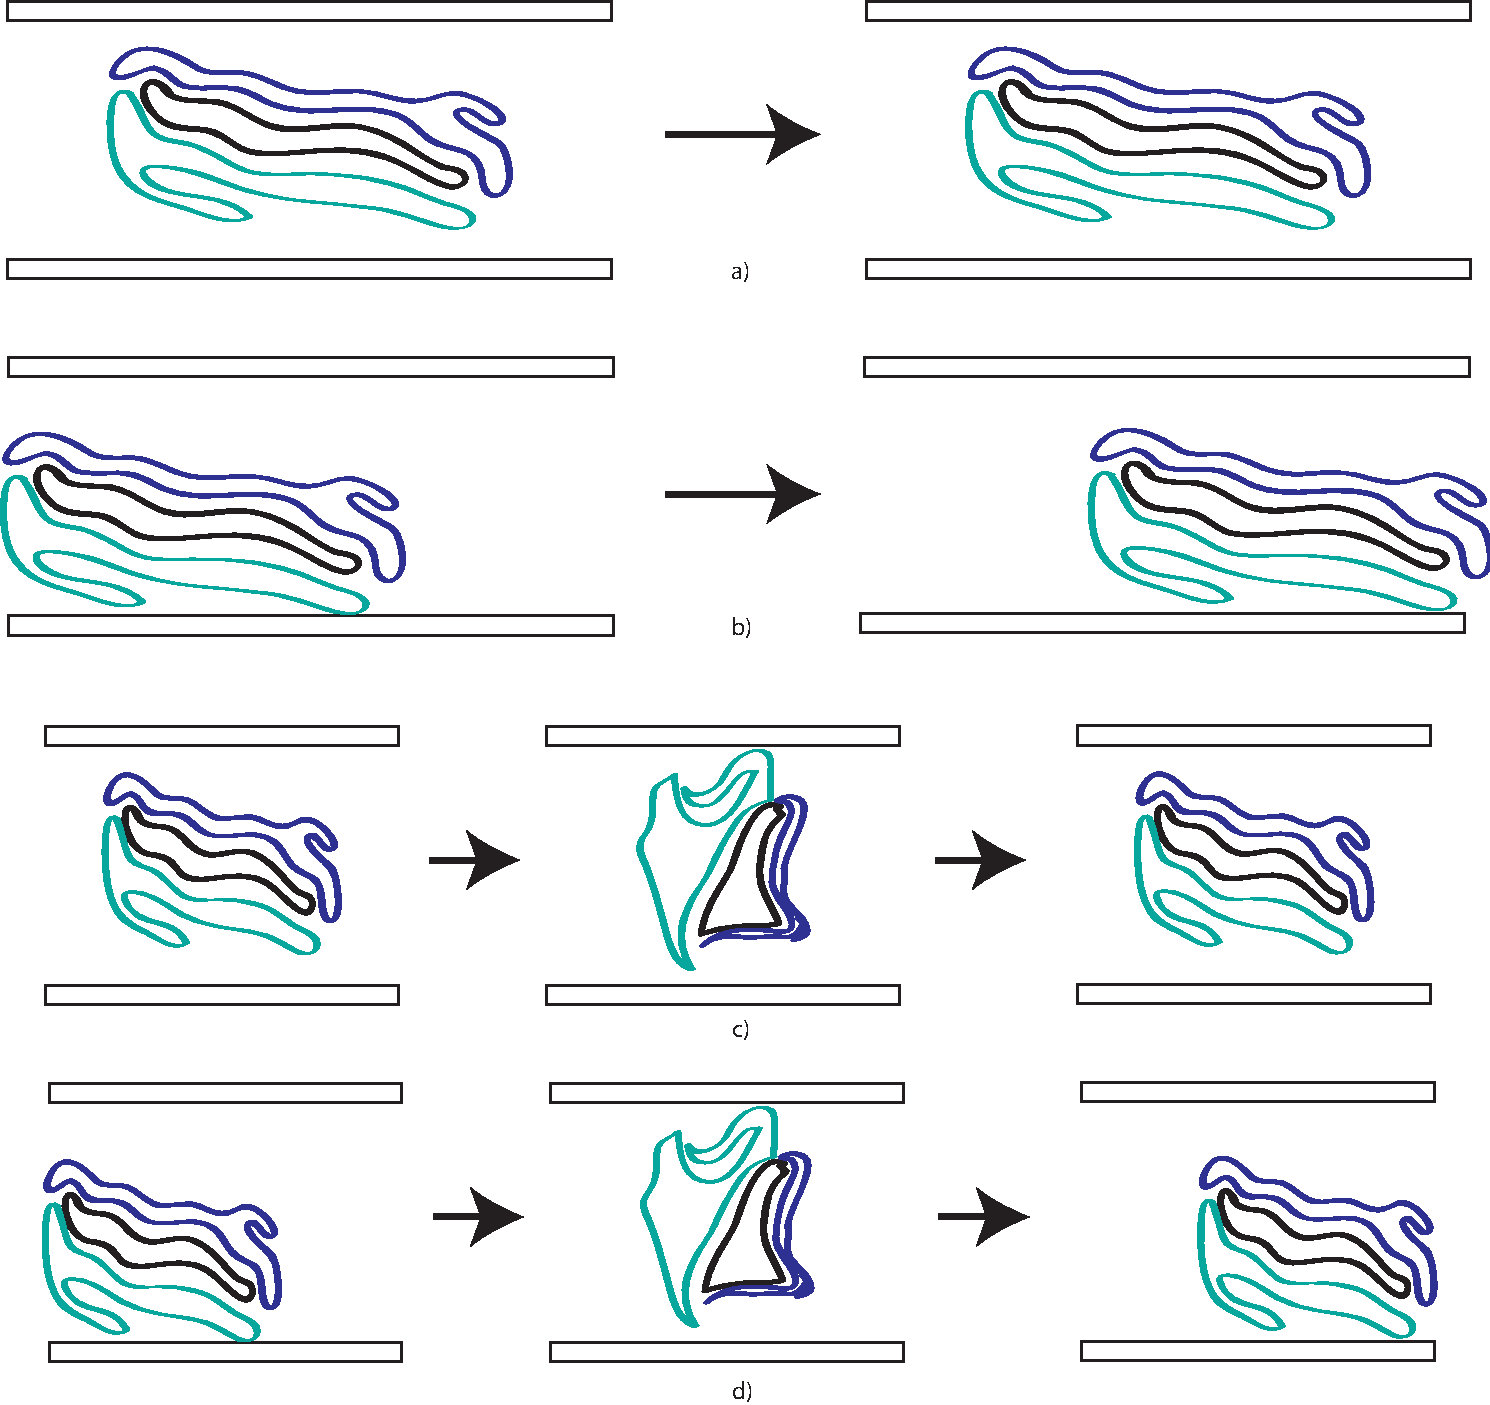
\includegraphics[scale=0.5]{Figs/ECSClassification}}
\caption[The four main categories of \ecs.]{The four main categories of \ecs. In all diagrams, only a particular flow structure is displayed, to demonstrate the various types of \ecs. These could be, for example, isosurfaces of velocity or energy. (a) An {equilibrium} solution, where the fluid structure does not change over time. (b) A {relative equilibrium} or {traveling wave} solution, where the state does not change in its own reference frame, but is translated relative to the observer. (c) A {periodic orbit}, where the flow state changes over time, but returns to the original state after some period $T$. (d) A {relative periodic orbit}, where the flow state is periodic in its own reference frame, but is translated relative to the observer.}\label{fig:ECS}
\end{figure}


Another avenue of research emerged in 1990, when Nagata computed nontrivial {\bf equilibrium} flow states for \pCf\ by continuing the wavy vortex solution of Taylor-Couette flow\rf{Nagata1990}. This class of solutions, which were named {\bf exact coherent structures} by Waleffe\rf{Waleffe2001} are the result of calculating exact, invariant solutions of the fully resolved Navier-Stokes equations. The family of \ecs\ was expanded with the discovery of {\bf traveling wave equilibria} by Nagata in 1997, the computation of {\bf periodic orbits} by Kawahara and Kida in 2001\rf{Kawahara2001}, and the computation of {\bf relative periodic orbits}\footnote{That is, flow states that are periodic after some phase shift.} by Viswanath in 2007\rf{Viswanath2007}. \refFig{fig:ECS} summarizes these four categories of \ecs. The ultimate hope of this line of research is that turbulence can be viewed as chaotic trajectories on the inertial manifold that are guided by hyperbolic \ecs\footnote{That is to say, the \ecs\ have many stable directions that are highly attractive and pull trajectories towards them, and a few unstable directions that ultimately eject the trajectory.} (\refFig{fig:guidedTurbulence}). \\

\begin{figure}[h]
\centerline{
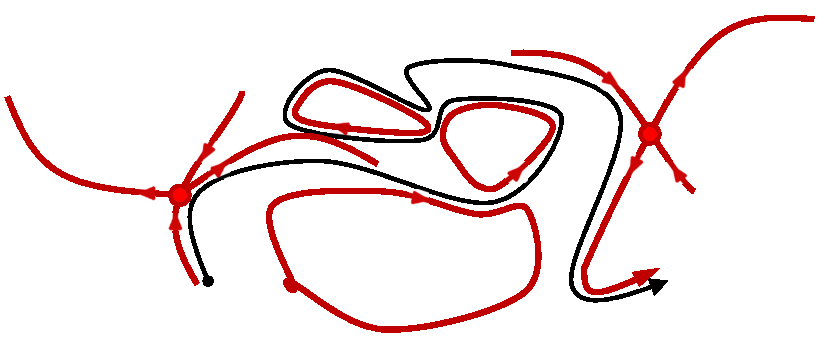
\includegraphics[width=\textwidth]{Figs/phaseSpaceTraj.pdf}}
\caption[A schematic of a turbulent trajectory in state space and the coherent structures that guide it.]{A schematic of a turbulent trajectory in state space and the coherent structures that guide it. (a) A turbulent trajectory in black appears chaotic and unpredictable in isolation. (b) When the underlying coherent structures in red are superimposed, however, the guiding of the dynamics by the \ecs\ becomes evident. Starting from the left, the trajectory is pulled in towards an equilibrium (filled circle) along its stable manifold (arrow pointing inwards), before being ejected along its unstable manifold (arrow pointing outwards). The trajectory then shadows three periodic orbits, whose stable and unstable manifolds are not trivial to represent visually, but nonetheless exist, before being attracted and ejected by the final equilibrium and continuing on its way. Reproduced from D. Borrero-Echeverry, \emph{Subcritical Transition to Turbulence in Taylor-Couette Flow}, PhD. Dissertation, Dept. of Physics, Georgia Institute of Technology, 2014\rf{Borrero2014}.}\label{fig:guidedTurbulence}
\end{figure}

\begin{figure}[t]
\centerline{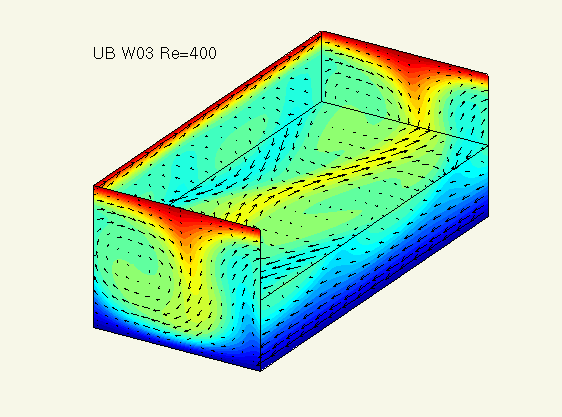
\includegraphics[scale=0.5]{Figs/rollStreak}}
\caption[The roll-streak structure of the Nagata upper branch equilibrium]{The roll-streak structure of the Nagata upper branch equilibrium\rf{Nagata1990}. The in-plane velocity vectors in the periodic cell are displayed for the box walls, as well as the mid-plane. The coloration reflects the streamwise velocity, where blue indicates a large streamwise velocity out of the page, and red represents a large streamwise velocity into the page. The vortex that forms the roll is clearly visible on the near box wall, as is the streak running through the midplane of the box. These structural features are often seen in real turbulent flows, and solutions that approach the vicinity of this solution in the state space will take on some of this roll-streak structure. Reproduced from J. F. Gibson, J. Halcrow and P. Civitanovi\'c, \emph{Visualizing the geometry of state space in plane Couette flow}, Journal of Fluid Mechanics, vol. 611, pp. 107-130, 2008\rf{Gibson2008}.}\label{fig:rollstreak}
\end{figure}


Of the work that has been done in the field, a large proportion of it has been computational, and experiments by Hof et al. and De Lozar et al.\rf{Hof2004,DeLozar2012} provide the only direct experimental verification of the existence of \ecs~in nature to date. However there have been several indirect results that establish the importance of \ecs\  in turbulent dynamics. These include the resemblance of Nagata's so-called `upper branch' equilibrium solution\rf{Nagata1990} to the roll-streak structure seen in DNS\rf{Gibson2008} (\refFig{fig:rollstreak}), and the potential role of the stable manifold of its sister lower branch solution in separating the turbulent and laminar basins of attraction\rf{Waleffe2001}. Advances in computing power, along with the development of CFD algorithms, such as {\tt Channelflow}\rf{Gibson2014}, have also made the computation of these structures generally feasible.\\

 In order to compute the first generation of \ecs, researchers placed substantial symmetry constraints on the dynamics. This had the benefit of greatly reducing the computational cost, but has resulted in \ecs\ that are not necessarily representative of turbulence, since we expect turbulent fields to display little to no symmetry in general. As a result, while the symmetric \ecs\ 	appear to inform our understanding of turbulent transitions\rf{Halcrow2008}, they do not necessarily inform our understanding of turbulent dynamics. The focus of this thesis has been to find periodic orbits with broken symmetry, and to investigate their properties and how they compare to their unbroken brethren.\\ 
 




In Chapter 1, I will lay out the Navier-Stokes equation and the Couette geometry  in further detail. In Chapter 2, I will discuss the symmetries of the Navier-Stokes equations for plane Couette flow and the advantages and disadvantages afforded by considering symmetric subspaces. Chapter 3 will discuss in detail the spectral methods used to integrate Navier-Stokes forward in time and the Newton-Krylov-hookstep algorithm used to find \ecs\ in {\tt Channelflow}, along with the workflow used in this thesis. Chapter 4 will present the results of these calculations, which include a new low-period orbit with broken symmetry that exists over a wide range of Reynolds numbers and computational domain sizes. Finally, Chapter 5 will provide a summary of the main ideas and suggests potential topics for future research. 
 
 
 
 
 

	\setcounter{secnumdepth}{3}
\chapter{Equations of Flow}
    	 	\epigraph{Peace is a lie, there is only passion. \\
			       Through passion, I gain strength.\\
			        Through strength, I gain power.\\
			        Through power, I gain victory.\\
			        In victory, my chains are broken.\\
                                        The Force shall set me free.}{Anonymous}
\section{Formalisms}
%At the heart of fluid dynamics lies the Navier-Stokes equation, first derived by George Stokes in 1845, after a series of refinements leading back to Newton.
If we were to describe the dynamics of a point particle, we would probably begin by writing the total force on the object as a sum of various contributions - thrust, drag, electric, magnetic, gravitational, etc., so that 
\begin{equation}
\Vector{F}_{\mathrm{total}} = \sum{i}{}{F_{i}}.
\end{equation}

To relate this back to the {\bf kinematic} variables (position, velocity, etc.), we can then use Newton's Second Law,
\begin{equation}\label{eq:NSL}
\der{1}{\Vector{p}}{t} = \Vector{F}_{total},
\end{equation}
to generate an equation of motion. The trajectory could then be calculated via analytic or numeric integration of \refeq{eq:NSL}. While in principle we can use this approach to describe the behavior of a large collection of particles making up the fluid, practical considerations prevent us from modeling the behavior of each individual particle, for the following reason -- in a milliliter of water, there are approximately $10^{22}$ molecules of water, each with 6 degrees of freedom.\footnote{If we ignore the vibrations of the O-H bonds} Applying \eqref{eq:NSL} to all these particles would result in about $10^{23}$ coupled ordinary differential equations. Such a set of equations would be hard to write down, let alone solve! Clearly, a more intelligent approach is needed. The formalism that I will present here begins by modeling the fluid as a continuum. My derivation is based off that in\rf{Granger1995}. \\

\subsection{The Eulerian Formulation}

When asked to consider the mechanical evolution of some collection of bodies, two obvious methods would be readily apparent - we could either follow a collection of particles on their way through space and time (the {\bf Lagrangian} formulation), or we could situate ourselves at some point in space and observe the properties of particles that pass through the surrounding region (the {\bf control volume}) over time (the {\bf Eulerian} formulation). The Lagrangian formulation will be familiar to anyone with a basic physics education, since it lends itself readily towards analysis of rigid-body motion. When considering fluids, however, the disadvantages of the Lagrangian formulation (noted above) stand in contrast to the ease of analysis afforded by the Eulerian formulation, which remains as easy (or hard) as it was for rigid body motion. For this reason, I will focus on the Eulerian formulation of fluid mechanics.

\subsection{The Fluid Particle}
A consequence of the Eulerian formulation is that we cannot know the full timeline of any individual particle over its lifetime -- we only know the properties of particles within the control volume. Therefore, the principle quantity in the Eulerian formulation is the {velocity field}\footnote{As opposed to particle trajectories $\Vector{x}(t)$ in the Lagrangian formulation.} $\Vector{v}(\Vector{x},t) = v_x(\Vector{x},t) \Vector{\hat{x}} + v_y (\Vector{x},t)\Vector{\hat{y}} + v_z(\Vector{x},t) \Vector{\hat{z}}$, along with the pressure and density fields, which are the average values of these properties in a control volume surrounding a point. \\

A subtle issue arises in doing this, however. Since the velocity field is continuous, it has a well-defined value at every point in space, which we would want to be associated with the velocity of a particle at that point in space. However, there are finite number of particles in any collection of fluid with a finite spatial extent. If these particles have some finite volume, then the formulation assigns multiple velocities to a single particle - and if the particles are infinitesimal, then the formulation assigns velocities to empty space! This issue can be resolved by appealing to the continuum hypothesis, which suggests that a control volume (the `{\bf fluid parcel}') can be chosen such that it is large enough to form a meaningful average of the quantities within, but small enough that the properties do not vary significantly over the parcel, and that from a macroscopic perspective, the properties appear continuous. \\

The reader may ask ``Can such a  parcel even exist?". As an example, let us consider water, with approximately $10^{22}$ molecules per cubic centimeter. Imagine our fluid parcels as tiling the volume with cudes with sides of length $dl$, giving a total volume of $dl^3$ per parcel. First, let us make $dl$ small enough that the macroscopic properties appear continuous - how about one micron? That gives the volume of a fluid particle as one cubic micrometer. For scale, consider that the volume of the human red blood cell ranges from 80-100 cubic micrometers\rf{Fischer1983} - this seems acceptably small for considering, say, the flow around a ship.\footnote{The validity of the continuum hypothesis is clearly dependent on the density of the fluid and the length scale of the phenomenon to be modeled, but holds up even for the sparse gas clouds of protoplanetary disks\rf{Clarke2007} or at the nanoscale{Dorf2006}.} The number of water molecules within each fluid parcel is then 
\begin{equation}
10^{22}dl^3 = 10^{22} \times 10^{-12} = 10^{10},
\end{equation}   
or about 10 billion water molecules, which is certainly sufficient to achieve a meaningful average. Having defined a fluid parcel in this way allows us to behave as if these macroscopic variables have well-defined values at every point in space, which greatly simplifies the following analysis. 

\section{Mass Conservation}
While not formally a part of the Navier-Stokes equation (which is a statement about conservation of linear momentum), conservation of mass is nevertheless essential in solving fluid problems, and will serve as a demonstration of the control volume method. Consider a volume $\Omega$ which is fixed in space, and has some mass density $\rho = \rho(\Vector{x},t)$ and some fluid velocity $\Vector{v} = \Vector{v}(\Vector{x} ,t)$ that are generically functions of time and space, allowing us to define the {\bf mass current density} $\Vector{m} = \Vector{v}\rho$. The mass contained within the volume $\Omega$ is then given by 
\begin{equation}
M = \int{\Omega}{}{\rho}{dV}.
\end{equation}
The flow of mass out of the volume through the surface $d\Omega$ of $\Omega$ is given by 
\begin{equation}
\mathcal{M}_{flow} = \int{d\Omega}{}{\Vector{m}\cdot\Vector{n}}{dA} = \int{\Omega}{}{\Div{\paren{\rho\Vector{v}}}}{dV},
\end{equation}
by the divergence theorem.  Now in classical physics, mass should not appear or disappear, so the sum of the rate of mass flow into (or out of) the volume and the rate of change of mass inside the volume $M_{encl}$ must be zero, giving
\begin{equation}
\pder{1}{M_{encl}}{t} + \mathcal{M}_{flow} = 0,
\end{equation}
\begin{equation}
\pder{1}{}{t}\paren{\int{\Omega}{}{\rho}{dV}} + \int{\Omega}{}{\Div{\paren{\rho\Vector{v}}}}{dV} =0.
\end{equation}
Since $\Omega$ is time-independent, the time derivative commutes with the integral, giving 
\begin{equation}
\int{\Omega}{}{\pder{1}{\rho}{t} + \Div{\paren{\rho\Vector{v}}}}{dV} = 0.
\end{equation}
But $\Omega$ is arbitrary, so the integrand must be zero everywhere, and mass is conserved if
\begin{equation}\label{eq:consMassFull}
\pder{1}{\rho}{t} + \Div{\paren{\rho\Vector{v}} }= 0.
\end{equation}

If the flow is (approximately) incompressible, which will be true for small Mach numbers\footnote{The Mach number is the ratio of the fluid velocity to the speed of sound in the fluid. For reference, the speed of sound in water is 1497 ms$^{-1}$ at room temperature and pressure.}, then $\rho$ must be constant, and \refeq{eq:consMassFull} becomes 
\begin{equation}\label{eq:consMassIncomp}
\Div{\Vector{v}} = 0.
\end{equation}

\section{Conservation of Linear Momentum} 

As mentioned earlier, the Navier-Stokes equations are simply a statement of conservation of linear momentum, along with certain assumptions about stress  and strain, which are presented below. 
\subsection{Stress}

Stress is a mathematical entity that contains information about the forces acting on an object. As with force, we define positive stress as stress that acts towards the control volume, and negative if it acts away from it. Unlike force however, stress is not a vector, since it encodes both the force on an object, as well as the plane that force acts in. Since there are three directions and three planes of action, a stress entity generally has nine elements, and can be represented as a {\bf second rank tensor}. For example, the viscous stress tensor $\Tensor{T}$ is identified by two subscripts, where the first subscript indicates the plane of action, and the second the direction of action. So $\Tensor{T}_{xy}$ would represent the viscous force on the $(y,z)$ plane acting in the $y$ direction. 

\subsection{Strain}
Now that we can consider the forces on a fluid particle, we need to link these forces back to the observable quantities in the form of strain, a second rank tensor which encodes information about the deformation of the fluid packet. In solids, this is easy - Hooke's Law for elastic substances, for instance, sets the strain proportional to the stress:
\begin{equation}
\Vector{\sigma} = \Tensor{C}\Vector{\epsilon},
\end{equation}
where $\Vector{\sigma}$ is the Cauchy stress tensor, $\Tensor{C}$ is the (fourth rank) stiffness tensor and $\Vector{\epsilon}$ is the infinitesimal strain tensor. However, for fluids, this is not the case - you can imagine that if you applied a constant force to a cube of water, it would deform continuously, without offering any resistance. Newton theorized that for continuously deformable fluids, the 1-D relationship between stress $\Tensor{T}$ and strain $\Tensor{S}$ should have the following form:
\begin{equation}
\mu \der{1}{\Tensor{S}}{t} = \mu \der{1}{u}{x}=\Tensor{T}, 
\end{equation}
where $\mu$ is the fluid viscosity and $u$ is the velocity.  Stokes extended this to three dimensions, giving the Newtonian constitutive relationship between stress and strain (for an incompressible fluid):
\begin{equation}\label{eq:constitutive}
\Tensor{T}_{ij} = -P\delta_{ij} + \mu\paren{\pder{1}{u_{i}}{x_j} + \pder{1}{u_j}{x_i}},
\end{equation}
where $\delta_{ij}$ is the Kronecker delta function\footnote{$\delta_{ij} = 1$ if $i=j$ and $0$ otherwise} and $P$ is the pressure. A fluid obeying Newton's constitutive relation is called a Newtonian fluid. Water, and most gases under normal conditions are Newtonian, but fluids like blood, quicksand and corn starch (to name a few) are not. In this thesis, we will restrict ourselves to Newtonian fluids.

\subsection{Surface Forces}
Having written down the stress tensor $\Tensor{T}$ as a function of the velocity field, we can now link it to the surface forces on a fluid particle. Recalling that stresses act over $d\Omega$ of the fluid particle, the total surface force from stress is then simply 
\begin{equation}\label{eq:surfaceForce}
\Vector{F}_s = \int{d\Omega}{}{\Tensor{T}\cdot\Vector{n}}{dA},
\end{equation}
where $\Vector{n}$ is the surface normal. 
\subsection{Newton's Second Law}
For a fluid parcel $\Omega$, Newton's Second Law can be rewritten as
\begin{equation}\label{eq:NSLInt}
\sum{}{}{\Vector{F}}_{\mathrm{total}} = \int{\Omega}{}{
							\pder{1}{\rho\Vector{u}}{t}}{dV}
\end{equation}
where the sum is over all possible external forces. We can further split $\Vector{F}$ into two kinds of forces - body forces, like gravity or electromagnetism, and surface forces from stresses. We group the body forces $\Vector{F}_b$ as \begin{equation}
\Vector{F}_b = \int{\Omega}{}{\rho\Vector{f}}{dV},
\end{equation}
where $\Vector{f}$ is the {\bf body force density}. Using \refeq{eq:surfaceForce} to express the surface forces, \refeq{eq:NSLInt} becomes
\begin{equation}
\int{\Omega}{}{\rho{\Vector{f}-\pder{1}{\rho\Vector{u}}{t}}}{dV} + \int{d\Omega}{}{\Tensor{T}\cdot\Vector{n}}{dA} = 0.
\end{equation}
This can be written in differential form using the same trick used to generate \refeq{eq:consMassFull}, giving Cauchy's Equation of Motion
\begin{equation}\label{eq:CauchyEOM}
\rho{\Vector{f}-\pder{1}{\rho\Vector{u}}{t} } + \Div{\Tensor{T}} = 0.
\end{equation}
From this, the incompressible Navier-Stokes equation arise by a substitution of \refeq{eq:constitutive} into \refeq{eq:CauchyEOM}, giving (after tedious rearrangement by components),
\begin{equation}\label{eq:NS}
\pder{1}{\Vector{u}}{t} + \paren{\Vector{u}\cdot\nabla}\Vector{u} = \Vector{f} - \frac{1}{\rho}\Grad{P} + \frac{\mu}{\rho}\nabla^2\Vector{u}.
\end{equation}

By using the substitutions
\begin{align}
\Vector{x} &\Rightarrow L\Vector{x}\\
\Vector{u} &\Rightarrow U\Vector{u}\\
t &\Rightarrow \frac{L}{U}t\\
P &\Rightarrow \rho U^2P,
\end{align}
and neglecting body forces, we obtain the nondimensional version of \refeq{eq:NS} --
\begin{align}
\pder{1}{\Vector{u}}{t} + \paren{\Vector{u}\cdot\nabla}\Vector{u} = -\Grad{P} + \frac{1}{\ReN}\nabla^2\Vector{u}\label{eq:NSND},\\
\nabla\cdot \Vector{u} = 0,
\end{align}
where \begin{equation}\label{eq:ReN}\ReN= \frac{UL\rho}{\mu}.\end{equation} In practice, the values of $L$ and $U$ are chosen by convention to reflect the natural scales of the problem at hand.
 
\section{Plane Couette Flow}
Since \pCf\ is a shear driven flow, we set the pressure gradient to zero and use no-slip boundary conditions at the walls, which sets the surface tangential velocity equal to the surface velocity. The Navier-Stokes equation for \pCf\ is then given by 
\begin{equation}\label{eq:NSPCF}
\pder{1}{\Vector{u}}{t} + \paren{\Vector{u}\cdot\nabla}\Vector{u} = \frac{1}{\ReN}\nabla^2\Vector{u},
\end{equation}
with boundary conditions 
\begin{equation}\label{eq:PCBC}
\Vector{u}(x,\pm1,z,t) = \paren{\pm1,0,0},
\end{equation}
and geometry as pictured in \refFig{fig:planeCouette}. We nondimensionalize by the velocity $V$ of either plate and the half-plate distance $h$, with the Reynolds number
\begin{equation}
\ReN = \frac{hV\rho}{\mu}.
\end{equation} In order to derive the laminar velocity profile shown in \refFig{fig:planeCouetteBulk}, note that at very low \ReN, the right hand side of \refeq{eq:NSPCF} dominates. If we assume that the flow is unidirectional and steady, so that $\Vector{u} = u_x \Vector{\hat{x}}$, symmetry considerations tell us that the velocity field can only be a function of height, so that the Navier-Stokes equation reduces to 
\begin{equation}
\pder{2}{u_x}{y} = 0.
\end{equation}
This has a solution of the form
\begin{equation}
\Vector{u}(y) = y\Vector{\hat{x}},
\end{equation}
which corresponds to the laminar flow profile shown in \refFig{fig:planeCouetteBulk}. Consider then a perturbation $\Vector{v}(x,y,z,t)$ away from the laminar state, so that the initial field is $\Vector{u}(x,y,z,t) = \Vector{v} (x,y,z,t)+ y\Vector{\hat{x}}$. Substituting this into \refeq{eq:NSND}, we get 
\begin{align}
\pder{1}{\Vector{v}}{\tau} + y\pder{1}{\Vector{v}}{x} + v\Vector{\hat{x}} + \Vector{v}\cdot\Grad{\Vector{v}} &= \frac{1}{\ReN} \nabla^2\Vector{v},\label{eq:PertND}\\
\Div{\Vector{v}} &= 0.
\end{align}
Adapting the no-slip boundary conditions from \refeq{eq:PCBC}, we get
\begin{equation}
\Vector{v}(x,\pm 1,z,t) = 0.
\end{equation}
At this point we need to introduce artificial boundary conditions to  render the infinite planar domain into a computationally tractable form. We use the periodic boundary conditions 
\begin{align}
\Vector{v}(x,y,z,t) = \Vector{v}(x+L_x,y,z,t),\label{eq:periodicBCx},\\
\Vector{v}(x,y,z,t) = \Vector{v}(x,y,z+L_z,t),\label{eq:periodicBCz},
\end{align}
where $L_x$ and $L_z$ are the lengths of the periodic cell. This gives the complete equation of motion for the perturbing velocity field.  Since the laminar profile is steady, understanding the turbulent field's trajectory in state space now reduces to understanding the behavior of the turbulent perturbation, and the structure of its inertial manifold. \refeq{eq:pertND} is not generally analtyically integrable, so we must tackle it numerically. Before presenting the numerical methods and workflow, however, I will take a slight detour to discuss in detail the symmetries of the \pCf problem, as they are central to this thesis. 


	\chapter{Symmetry in \pCf}	
\epigraph{Tyger! Tyger! burning bright, \\
		In the forests of the night. \\
		What immortal hand or eye,\\
		Could frame thy fearful symmetry?}{William Blake, \emph{The Tyger}} 
Dynamical systems in physics often display symmetry. The electron wavefunction in hydrogen, or the gravitational motion of a planet around a star, for instance, display very high degrees of spatial symmetry.  Understanding the symmetries of a system can be incredibly useful to an investigator, since they hint at conserved physical quantities (through Noether's Theorem), and can greatly reduce the complexity of the system in various ways. Before I begin the discussion of the symmetries of \pCf, I will first define what `symmetry' means in this thesis. A system is said to be {\bf equivariant} under a symmetric transformation of the dynamical system if a transformation that commutes with the time evolution of the system - that is, for a symmetric transformation $S$ and a dynamical system $\dot{x} = f(x)$, $S \dot{x} = Sf(x) = f(Sx)$ implies that the system is equivariant under $S$. 

The symmetry relations of \pCf have been derived extensively in \cite{GIBSON2009}, which I will present here for the sake of flow\footnote{haha}. 
\section{Unbounded Navier-Stokes}

If we do not impose boundary conditions on the Navier-Stokes equations on an infinite domain, the system will be equivariant under continuous rotational and translational symmetry, as well as the discrete {\bf pointwise inversion} symmetry$\sigma_{xz}$, which has the following action on the system:

\begin{equation}\label{eq:pointwiseinversion}
\sigma_{xz}\Vector{u}\paren{\Vector{x}} = -\Vector{u}\paren{-\Vector{x}}
\end{equation}

While the rotation or translation transformation can be easily conceptualized, the pointwise inversion can provide some difficulty. The easiest way of visualizing the transformation is to view it in a 2D domain instead of in the full 3D, as shown in \figureref{fig:pointwiseinversion}. The proof of the equivariance of these transformations can be found in \cite{a}.



\section{Plane Couette Flow}

If the domain is limited to $\mathbb{R}^2 \times [-1,1]$ with the boundary conditions of \pCf, we lose some of the equivariant transformations of the full, unrestricted problem, leaving us with two basic discrete symmetries: a rotation by $pi$ about the $z$ axis (denoted $\sigma_x$ and a reflection about the $z$ axis (denoted $\sigma_z$)\footnote{The motivation for these subscripts will become apparent shortly}, with together form a discrete symmetry group $D = D_1 \times D_1 = \{e, \sigma_x,\sigma_z,\sigma_{xz}\}$ of order 4, where

\begin{align}\label{eq:discretesymm}
\sigma_x [u,v,w](x,y,z) &= [-u,-v,w](-x,-y,z)\\
\sigma_z [u,v,w](x,y,z) &= [u,v,-w](x,y,-z)\\
\sigma_{xz} [u,v,w](x,y,z) &= [-u,-v,-w](-x,-y,-z)
\end{align}

The continuous symmetries are the two parameter steamwise-spanwise translations, which, when provided periodic boundary conditions, form a continuous $SO(2)\times SO(2)$ symmetry group 
\begin{equation}\label{eq:contsymm}
\tau(l_x,l_z)[u,v,w](x,y,z) = [u,v,w](x+l_x,y,z+l_z).
\end{equation}

The group $\Gamma$ of equivariant solutions is then any combination of these symmetry operations, given by $\Gamma = SO(2)_x \ltimes D_{1,x} \times SO(2)_z \ltimes D_{1,z}$\footnote{$\ltimes$ is the semidirect product}. For a solution $\Vector{u}$ of \pCf, the group $s$ of symmetries that satisfies $s\Vector{u} = \Vector{u}$ is called the isotropy subgroup of $\Vector{u}$ and is said to fix $\Vector{u}$. Examples of such groups include the identity group $\{e\}$, which is typically the isotropy subgroup of turbulent solutions. Before I discuss the isotropy subgroup considered for this thesis, however, I will first highlight the useful properties of some particular symmetry subgroups to motivate the eventual choice of isotropy subgroup. 

\section{Properties of $\Gamma$}

It should be evident that since \pCf is equivariant under the continuous translations given in \eqref{eq:contsymm}, trajectories can be traveling wave equilibria or relative periodic orbits: that is, if one moves into a different inertial frame, the trajectory is a regular equilibrium or periodic orbit. However, an initial condition that is fixed by $\sigma_z$ cannot be translated in the spanwise direction without losing $\sigma_z$ symmetry (except for the trivial case where $\pder{1}{\Vector{u}_z}{z} = 0$). Similarly, an initial condition that is fixed by $\sigma_x$ cannot be translated in the streamwise direction without losing $\sigma_x$ symmetry (and an initial condition that is fixed by$\sigma_{xz}$ symmetry cannot be translated at all without losing $\sigma_{xz}$ symmetry). Since these symmetries are also invariant\footnote{That is, if the symmetry is satisfied at time $t = t_0$, it must be satisfied for all times.}, a trajectory with one of the discrete symmetries cannot have traveling waves in the direction corresponding to its subscript. \\

The presence of the periodic boundary conditions also implies that all solutions are fixed by the full-period translation $\tau(L_x,0)$ and $\tau(0,L_z)$. However, solutions can also be fixed by any rational translation of the form $\tau(\dfrac{m}{n}L_x,\dfrac{m'}{n'}L_z$, or by the continuous translations. In the latter case, the velocity field is necessarily constant along the translation direction, but in the former, it implies that the periodic cell is subdivided into repeating subcells. In this case, we can simply reduce the domain to the subcell, which implies that we need not fix $\Vector{u}$ under any translational symmetry other than the full period relation, which is required by the boundary conditions. \\

Finally, we can reduce the number of unique subgroups of $\Gamma$ by considering its {\bf conjugacy groups}. A group $N$ and $M$ are considered conjugate if for some $s \in \Gamma$, $N = s^{-1}Ms$ - that is, $N$ and $M$ are related by a coordinate transformation. This allows us to consider only one group out of a set of mutually conjugate groups (known as a conjugacy class), since any other group in the class is simply related by the application of a symmetry transformation. This becomes especially important when considering $O(2) =  SO(2) \ltimes D_{1}$, since it is not an abelian group as reflections and translations about the same axis are noncomutative (\figureref{fig:notabelian}). However, we can still recover a psuedo-commutative relation by considering \figureref{fig:notabelian}. We can see that $\sigma_z\tau_z$ results in the object moving by $l_z$ to the right, and the being mirrored across the $z$ axis, at which point it is mirrored and $l_z$ to the left of the origin. We can achieve the same effect by mirroring the object and moving it to the left - that is, applying the operation $\tau_z^{-1}\sigma_z$, leading us to conclude that $\sigma\tau = \tau^{-1}\sigma$. We can rewrite this as $\sigma\tau^2 = \tau^{-1}\sigma\tau$, so
\begin{equation}
\sigma_x\tau(l_x,0) = \tau^{-1}(l_x/2,0)\sigma_x\tau(l_x/2,0),
\end{equation}

which implies that $\sigma_x$ and $\sigma_x\tau_x$ are part of the same conjugacy class - so if a isotropy group contains $\sigma_x\tau_x$, there is a simpler version of that group which contains $\sigma_x$ instead. Note that if $l_x = L_x$, then we have $\sigma_x = \tau_x^{-1}\sigma_X\tau_x$, so reflection and translations commute for any half-integer cell shifts. In this thesis, I will work with either half-cell or or null shifts. The group of half cell shifts is denoted $C_2$, so the group 
\begin{align}
G &= D_{1,x} \times C_{2,x} \times D_{1,z} \times C_{2,z} \subset \Gamma
\end{align} 

is an abelian group of order 16, containing both the isotropy groups of half-cell and null shifts.

\section{Symmetry Groups of this Thesis}

We can categorize the conjugacy classes of $G$ by their order - in this thesis, we will work with order 2 and 4 classes. There are 15 subgrups of order-2 (since there are 15 non-identity elements in $G$), 35 subgroups of order 4 ($(15\cdot14) /(3\cdot2)$), 15 subgroups of order 8 and 1 subgroup of order 16, giving 67 subgroups of $G$. Luckily, the existence of conjugacy classes allow us to greatly simplify the number of distinct groups we need to consider. For order-2 subgroups, conjugacy between $\sigma_x$ and $\sigma_x\tau_x$ and $\sigma_z\tau_z$ allows us to simplify down to just 8 distinct groups, which are generated by $\sigma_x,\sigma_z,\sigma_{xz},\sigma_x\tau_z,\sigma_z\tau_x,\tau_x,\tau_z,\tau_{xz}$. Recalling the behavior of these symmetries, we can see that only $\sigma_{xy}$ generates a group without travelling waves, $\sigma_z$ and $\sigma_z\tau_x$ generate groups that allow travelling waves in the $x$ direction, $\sigma_x\tau_z$ and $\sigma_x\tau_z$ generate groups that allow travelling waves in the $z$ direction, and the pure translations allow travelling waves in any (in-plane) direction. \\

  


	\chapter{Numerics and Workflow}

    	 	\epigraph{On two occasions I have been asked, ``Pray, Mr. Babbage, if you put into the machine wrong figures, will the right answers come out?" ... I am not able rightly to apprehend the kind of confusion of ideas that could provoke such a question.}{Charles Babbage, Passages from the Life of a Philosopher}

Computational studies of Navier-Stokes, especially as a dynamical system, are difficult for many reasons, but most important among them is the high degree of complexity inherent in the numerical tools required to maintain efficiency. As mentioned earlier, the two major approaches towards simulating Navier-Stokes are modeling, where some assumptions are made to reduce the difficult of simulation, and direct numerical simulation (DNS), where no assumptions beyond those used to derive Navier-Stokes and set up the boundary conditions are used. DNS is naturally more accurate (since the physicality of some modeling assumptions can be suspect), but since it fully resolves Navier-Stokes, it is significantly more expensive than modeling, and methods that attempt to offset this extra cost tend to be extremely complex. For this reason, I use the open source library {\tt Channelflow}\rf{Gibson2014}, which has been essential in making any headway in this thesis. {\tt Channelflow} is a spectral DNS library, with additional utilities to find, parametrically continue, and analyze \ecs, which I will lay out in some detail below.
\section{The Spectral Method}
\subsection{The Residual}

Spectral methods are, like finite element methods, part of a larger class of numerical methods known as {\bf weighted residual methods}. In this class of methods, functions are approximated by a truncated series expansion, with the restriction that a quantity related to the residual be zero (instead of the residual itself). The quantity used for the spectral method is the scalar product 
\begin{equation}\label{eq:scalarProduct}
\scprod{u}{v}{w} = \int{a}{b}{uvw}{dx},
\end{equation}
where  $u(x),v(x)$ are some functions on the interval $[a,b]$, and $w(x)$ is a weighting function. If we then imagine some platonic function\footnote{That is, the function that is to be approximated} $u(x)$ that we attempt to approximate via a finite series expansion, so that
\begin{equation}\label{eq:seriesExpansion}
u_N(x) = \sum{k=0}{N}{\hat{u}_k \psi_k(x)},
\end{equation}
for some set of orthogonal basis functions $\psi_k(x)$, then the residual is given by
\begin{equation}
R_N = u(x)-u_N(x),
\end{equation} 
and for some differential equation
\begin{equation}
Du = f,
\end{equation}
where $D$ is some arbitrary differential operator and $f(x)$ is some arbitrary source function, the residual is defined
\begin{equation}
R_N = Du_N,
\end{equation}
as expected. While it may seem logical to require $R_N = 0$, this is not possible in general for finite $N$, so we instead require that for a set of test functions $\phi_i(x)$ and weighting function $w^*$, 
\begin{equation}\label{eq:SpectralZero}
\scprod{R_N}{\phi_i(x)}{w^*} = R_N(x_i) = 0,
\end{equation}
for some set of $x_i$. If $\phi_i(x) = \delta(x-x_i)$ and $w^* = 1$, then we have the colocation method, which forces the approximation to match the platonic function at a set of points. If $\phi_i(x) = \psi_i(x)$ and $w^* = w$, then we have the Galerkin method, which forces the mean residual to be zero. 

\subsection{Basis Functions}

In the spectral method, the basis functions are trigonometric functions. The advantage of trigonometric functions over polynomials is the rapid convergence of the series coefficients -- the Fourier coefficients converge exponentially fast, so we can achieve extremely high accuracy with a lower number of modes\rf{Peyret2002}.\footnote{Spectral methods are inappropriate when the boundary geometry is highly complex, as is the case in the majority of industrial applications, where more general finite element methods are used.} {\tt Channelflow} uses Fourier series in the streamwise-spanwise directions, where the basis functions and spectral projection are given by 
\begin{align}
F_k(x) = \exp{ikx}\\
u_K(x) = \sum{k=-K}{K}\hat{u}_k\exp{ikx},
\end{align}
and Chebyshev polynomials of the first kind in the wall-normal direction, where the basis functions and spectral projection are given by
\begin{align}
T_k(x) = \cos{k\arccos{x}}\\
u_N(x) = \sum{k=0}{(2k-1)/2}\hat{\mathfrak{u}}_kT_k(x).
\end{align}
\par The Fourier series expansion is particularly nice since the derivative $\partial_x F_k(x) = ikF(x)$ is especially easy to calculate, as are the Fourier coefficients by virtue of the Fast Fourier Transform, implemented in the Fastest Fourier Transform in the West (FFTW)\rf{Frigo1998}.\\

For Chebyshev polynomials, the derivative is slightly more complicated, since 
\begin{equation}
\partial_x T_k(x) = 2k\sum{n=0}{K}{\frac{1}{c_{k-1-2n}} T_{k-1-2n}(x)},
\end{equation}
where $c_k = 1$ if $k=1$ and $2$ if $k > 1$. Since the derivative of a single Chebyshev term becomes a sum of Chebyshev terms, the derivative of the Chebyshev representation of a function 
\begin{align}
\partial_x \sum{k=0}{N}\hat{\mathfrak{u}}_kT_k(x) &= \sum{k=0}{N}\hat{\mathfrak{u}}_k^{(1)}T_k(x),\\
\hat{\mathfrak{u}}_k^{(1)} &= \frac{2}{c_k}\sum{\substack{p = k+1\\(p+k) \mathrm{~odd}}}{N} p \hat{\mathfrak{u}}_p, \hspace{0.25cm} k \neq N,\\
\hat{u}^{(1)}_N &= 0.
\end{align}
As with the Fourier decomposition, however, Chebyshev coefficients can be calculated by a discrete cosine transform\rf{Halcrow2008}, which is a special case of the discrete Fourier transform, and is thus also computed by FFTW. 

While Fourier expansions are the easiest to deal with, they are best used on periodic boundaries, since the imposition of aperiodic boundary conditions on a Fourier series expansion can lead to Gibbs oscillations that can make the simulation aphysical\rf{Peyret2002}. For this reason, the velocity field is expanded as a Fourier series in the plane, and as a Chebyshev polynomial in the wall-normal direction. The velocity field is then represented as 
\begin{equation}
\Vector{u}_{KJL}(x,y,z) = \sum{k=-K}{K}{\hat{u}_k(x)\exp{ikx}}\sum{j=-J}{J}{\hat{u}_j(z)\exp{ijz}}\sum{l=0}{L}{\hat{\mathfrak{u}}_l(y)T_l(y)}.
\end{equation}

\subsection{Spatio-Temporal Discretization} 

Under the (Galerkin) spectral approximation 
\begin{equation}
\Vector{u}(x,y,z) = \Vector{U}_{KJL}(x,y,z),
\end{equation}
the partial differential equation
\begin{equation}
\pder{1}{\Vector{u}}{t} = f_T(\Vector{u}),
\end{equation}
becomes an ordinary differential equation (ODE)
\begin{equation}
\der{1}{\Vector{U_{KJL}}}{t} = F_T(\Vector{U}_{KJL}), 
\end{equation}
where $f_T(\Vector{u})$ is the forward time evolution of the Navier-Stokes equation, and $F_T(\Vector{U}_{KJL})$ is its spectral approximation via \refeq{eq:SpectralZero}. The temporal ODE can be solved in any number of ways -- {\tt Channelflow} allows the user to choose from several implicit-explicit methods, where the implicit : Crank-Nicolson Forward Euler, Crank-Nicolson Adams-Bashforth, Spalart-Moser Runge-Kutta and Semi-implicit Backwards Differentiation of orders 1 to 4. The order 3 Semi-implicit Backwards Differentiation (SBDF3) was chosen by default, and no reason to change this was anticipated, since SBDF3 is known to have a relatively large time step and low error for large \ReN\rf{Ascher1995}.

\section{Newton-Krylov-Hookstep Method}

In order to find \ecs\, it is necessary to solve the equation
\begin{equation}\label{eq:NRResidual}
\Vector{u} - \sigma f_T(\Vector{u}) = R_T(\Vector{u}) = 0,
\end{equation}
which is easiest tackled by root-finding algorithms. The root finding method used by {\tt Channelflow} is based on Newton's method, with some additional refinements. \\
\subsection{Newton's Method}
The principle behind Newton's method is as follows: Suppose we have $f(x)$ be a smooth and differentiable function, and an initial, `good' guess\footnote{How good a guess needs to be is highly dependent on the problem. Through this thesis, an initial condition that gave $R_T(\Vector{u}) < 0.001$ was considered a sufficiently good guess.}  $x_0$ for the root of $f$. Then we can find a better guess for the root of $f$ by finding the root of the tangent line at $f(x_0)$ (\refFig{fig:Newton}). Mathematically, 
\begin{align}
f(x_n) + f'(x_n)\paren{x_{n+1} - x_n} = 0,\label{eq:NRS1D}\\ 
x_{n+1} = x_n - \frac{f(x_n)}{f'(x_n)}.\label{eq:NR1D}
\end{align}
In higher dimensions, \refeqs{eq:NRS1D}{eq:NR1D} are replaced by the matrix equations
\begin{align}
\Vector{f}(\Vector{x}_n) + \mathbb{J}_{f,\Vector{x_n}}(\Vector{x}_{n+1} - \Vector{x}_n) = 0,\label{eq:NRSND}\\
\Vector{x}_{n+1} = \Vector{x}_n - \mathbb{J}_{f,\Vector{x}_n}^{-1}\Vector{f}(\Vector{x}_n)
\end{align}
where $\mathbb{J}_{f,\Vector{x_n}}$ is the Jacobian of the Navier-Stokes equation at $\Vector{x}_n$.\\
 
Newton's method is extremely fast and converges quadratically on the root\rf{Press2007}, but is not guaranteed to do so - a simple example is if the $n$-th guess is at (or very close to) a local minimum, in which case the adjustment term of \refeq{eq:NR1D} will explode, taking us very far away from the initial, good guess. As a result, 
\begin{figure}[h]
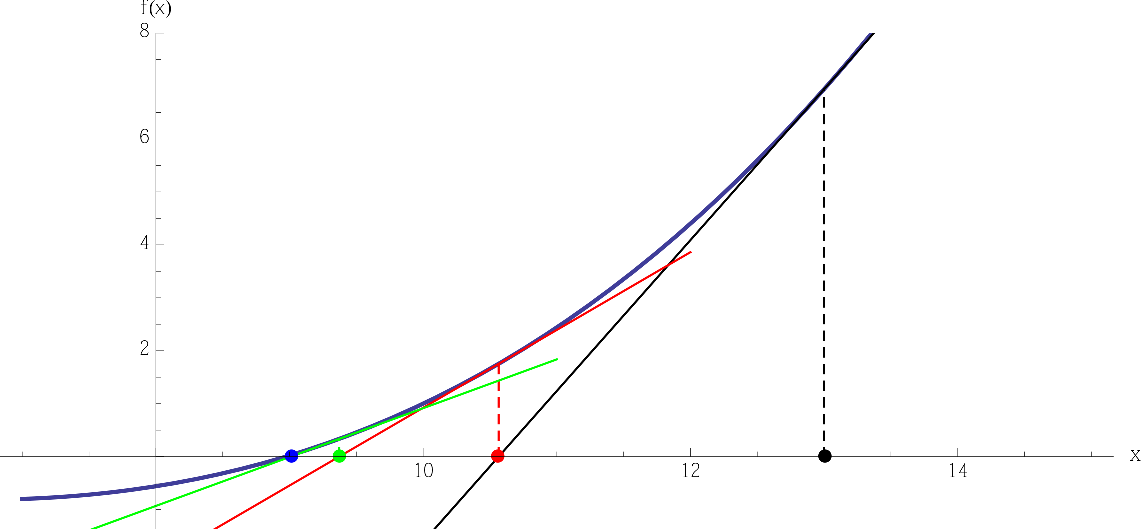
\includegraphics[width=\textwidth]{NRMethod}
\caption{A demonstration of Newton's method in 1D on a simple function with the root at $x_r \approx 8.98$. Starting at $x_0$ = 13, the method converges to $10^{-4}$ in just three steps.}\label{fig:Newton}
\end{figure}  




	\chapter{Results}
\epigraph{The first law of thermodynamics says that work cannot be destroyed. We who use computers know better.}{A frustrated Ph.D. candidate}

\section{The Gang of Four}

Four new periodic orbits P85, P60, P32 and P8 (\refFigsss{fig:p85}{fig:p60}{fig:p32}{fig:p8}), also known as the Gang of Four, have been found, with properties that are summarized in \refTab{tab:summary}.  We were unable to find any \ecs\ in asymmetric subspace. 

\begin{table}[h!]
\caption{A summary of relevant information regarding the Gang of Four. All of these results are presented at $\ReN = 400$, in the Hamilton-Kim-Waleffe cell\rf{Hamilton1995} with $(L_x,L_z) = (5.51157, 3.76239)$, and grid discretization $(N_x,N_y,N_z)= (48,33,48)$. The label for each orbit is based on its period, which experience shows uniquely defines an orbit. The phase velocities $v_x$ and $v_z$ are in terms of fraction of cell length per period. The largest Floquet exponent and number of unstable Floquet exponents are explained in a later section, as are the mean dissipation and energy input. The symmetry isotropy subgroup of each orbit is also provided. }   \label{tab:summary}
\begin{center}
\begin{tabular}{r   c  c  c  c  c  c  c  l }
\toprule
Label & $T$ & $v_x$ & $v_z$ &  $\lambda_{\textrm{max}}$ & $\#\ \lambda_{\textrm{unstable}}$ & $\bar{D}/\bar{I}$&  Symmetry \\
\midrule
\midrule
P85 & 85.50 & 0 & 0 & 0.0427 & 6 &1.85 & S\\

P60 & 60.86 & 0 & 0 &  0.032749 & 10 & 2.08 & S\\

P32 & 32.00 & 0.5 & 0 &  $0.0200 + 0.0982\imath$ & 7& 1.98 &$S_x$\\

P8 & 8.32 & 0 & $2.29\times 10^{-7}$ & $0.0998 - 0.2605 \imath$ &20& 4.00& $S_z$\\
\bottomrule
\end{tabular}
\end{center}
\end{table}
\subsection{Visualizations}   

Visualizing the behavior of fluids is in itself a time-honored discipline, especially when CFD is involved,\footnote{As the old joke goes, CFD really stands for {\bf C}olorful {\bf F}luid {\bf D}ynamics.} and well chosen visualization schemes can be, in and of themselves, an excellent tool for interpreting and analyzing data. Here, we use two main visualization methods.
\subsubsection{Orthographic Projection}
\refFigsss{fig:p85}{fig:p60}{fig:p32}{fig:p8} are all examples of the first visualization method -- the {\bf orthographic projection} (OP)\rf{Gibson2008}. The OP is constructed by piecing together several representative 2D slices of the state's velocity field -- each of the periodic boundaries, and the mid-plane, and is colored to represent the magnitude and direction of streamwise velocity. The OP allows us to visually interrogate the structure of the state, which can be extremely useful -- for example, it is clear purely from visual interrogation that \refFig{fig:p8} is less ordered than \refFig{fig:p85}. However, the OP cannot deliver much more than this -- for example, it cannot easily tell us much about the differences between the orbits of, say, P8 and P85. For this reason, we use the second, more useful visualization method - the state space projection\rf{Gibson2008}.
\begin{figure}
\centerline{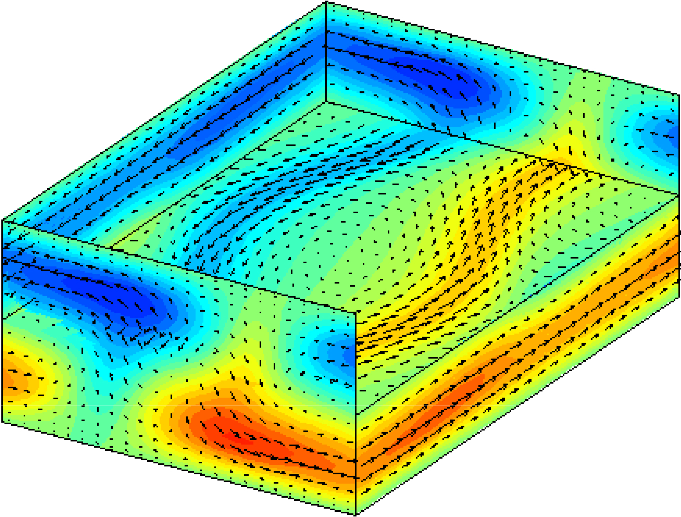
\includegraphics[width=\textwidth]{p85noBase.pdf}}
\caption{OP of P85. P85 is a fully symmetric orbit with period 85.50 in the HKW cell at $\ReN=400$. Note the extreme symmetry of the prominent streaks visible in the mid-plane. The velocity field pictured here is the turbulent perturbation only; the laminar flow has been subtracted away.{Available at {\tt http://goo.gl/hxRp8E}}}\label{fig:p85}
\end{figure}

\begin{figure}
\centerline{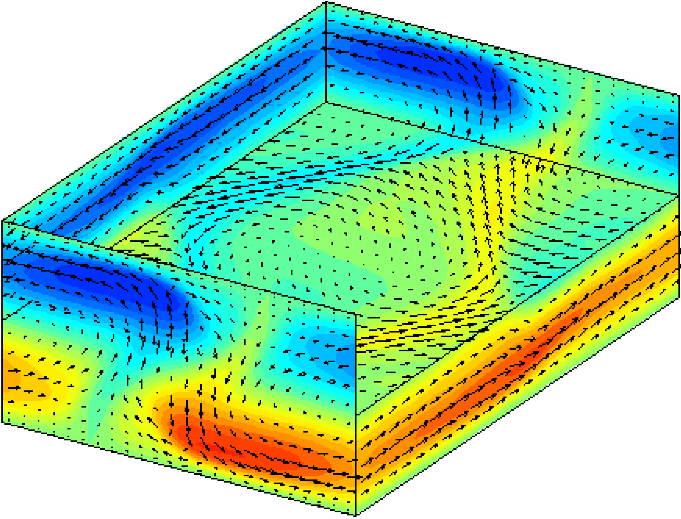
\includegraphics[width=\textwidth]{p60noBase.pdf}}
\caption{OP of P60. P60 is another fully symmetric orbit with period 60.86 in the HKW cell with $\ReN = 400$. While it displays an ellipsoid streak structure similar to P85, the energy of these streaks is lower.The velocity field pictured here is the turbulent perturbation only; the laminar flow has been subtracted away.{Available at {\tt http://goo.gl/4fQalm}}}\label{fig:p60}
\end{figure}


\begin{figure}
\centerline{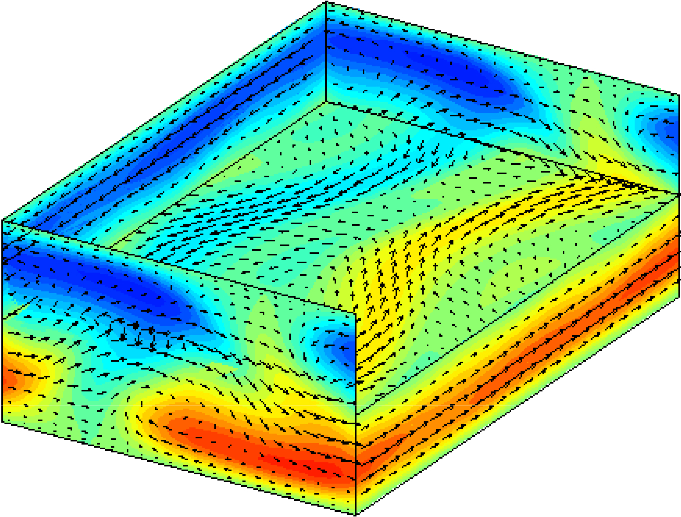
\includegraphics[width=\textwidth]{p32noBase.pdf}}
\caption{OP of P32. P32 is a streamwise asymmetric periodic orbit fixed by the symmetry group $S_z$, which is functionally a mirror symmetry about the streamwise axis. However, notice that while P32 does not \emph{exactly} maintain rotational symmetry about the streamwise axis, it bear remarkable similarity to P85 and P60. The rotational symmetry residual was $10^{-3}$, which is an few orders of magnitude lower than symmetries that are obviously not satisfied, but is not low enough ($10^{-6}$) to be accepted as a legitimate symmetry.  In the HKW cell at $\ReN=400$, the period is 32.00, and the streamwise relative velocity is $-0.5$ cell lengths per period.The velocity field pictured here is the turbulent perturbation only; the laminar flow has been subtracted away. Available at {\tt http://goo.gl/E8wRLm}}\label{fig:p32}
\end{figure}


\begin{figure}
\centerline{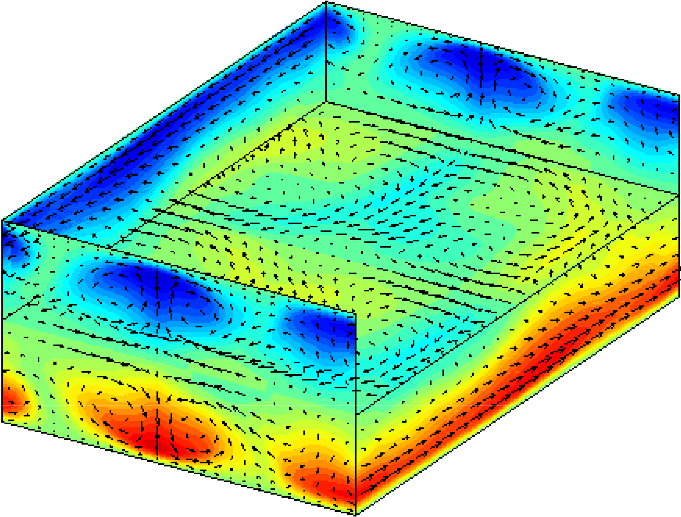
\includegraphics[width=\textwidth]{p8noBase.pdf}}
\caption{OP of P8. P8 is a spanwise asymmetric periodic orbit fixed by the symmetry group $S_x$, which is functionally a rotation by $\pi$ about the spanwise axis. In the HKW cell at $\ReN = 400$, the period is 8.32, and the spanwise relative velocity is $2.29\times 10^{-7}$ cell lengths per period. This number may seem low, but if it is not accounted for, the NKH solver cannot converge. P8 also has a rather short period, almost an order of magnitude shorter than most orbits recorded in the database at {\tt channelflow.org}. Since the Arnoldi iteration has a time cost that scales linearly with the period, P8 has been the least computationally demanding period orbit to analyze. The velocity field pictured here is the turbulent perturbation only; the laminar flow has been subtracted away. Available at {\tt http://goo.gl/uTDrLw}}\label{fig:p8}
\end{figure}



\begin{figure}[h]
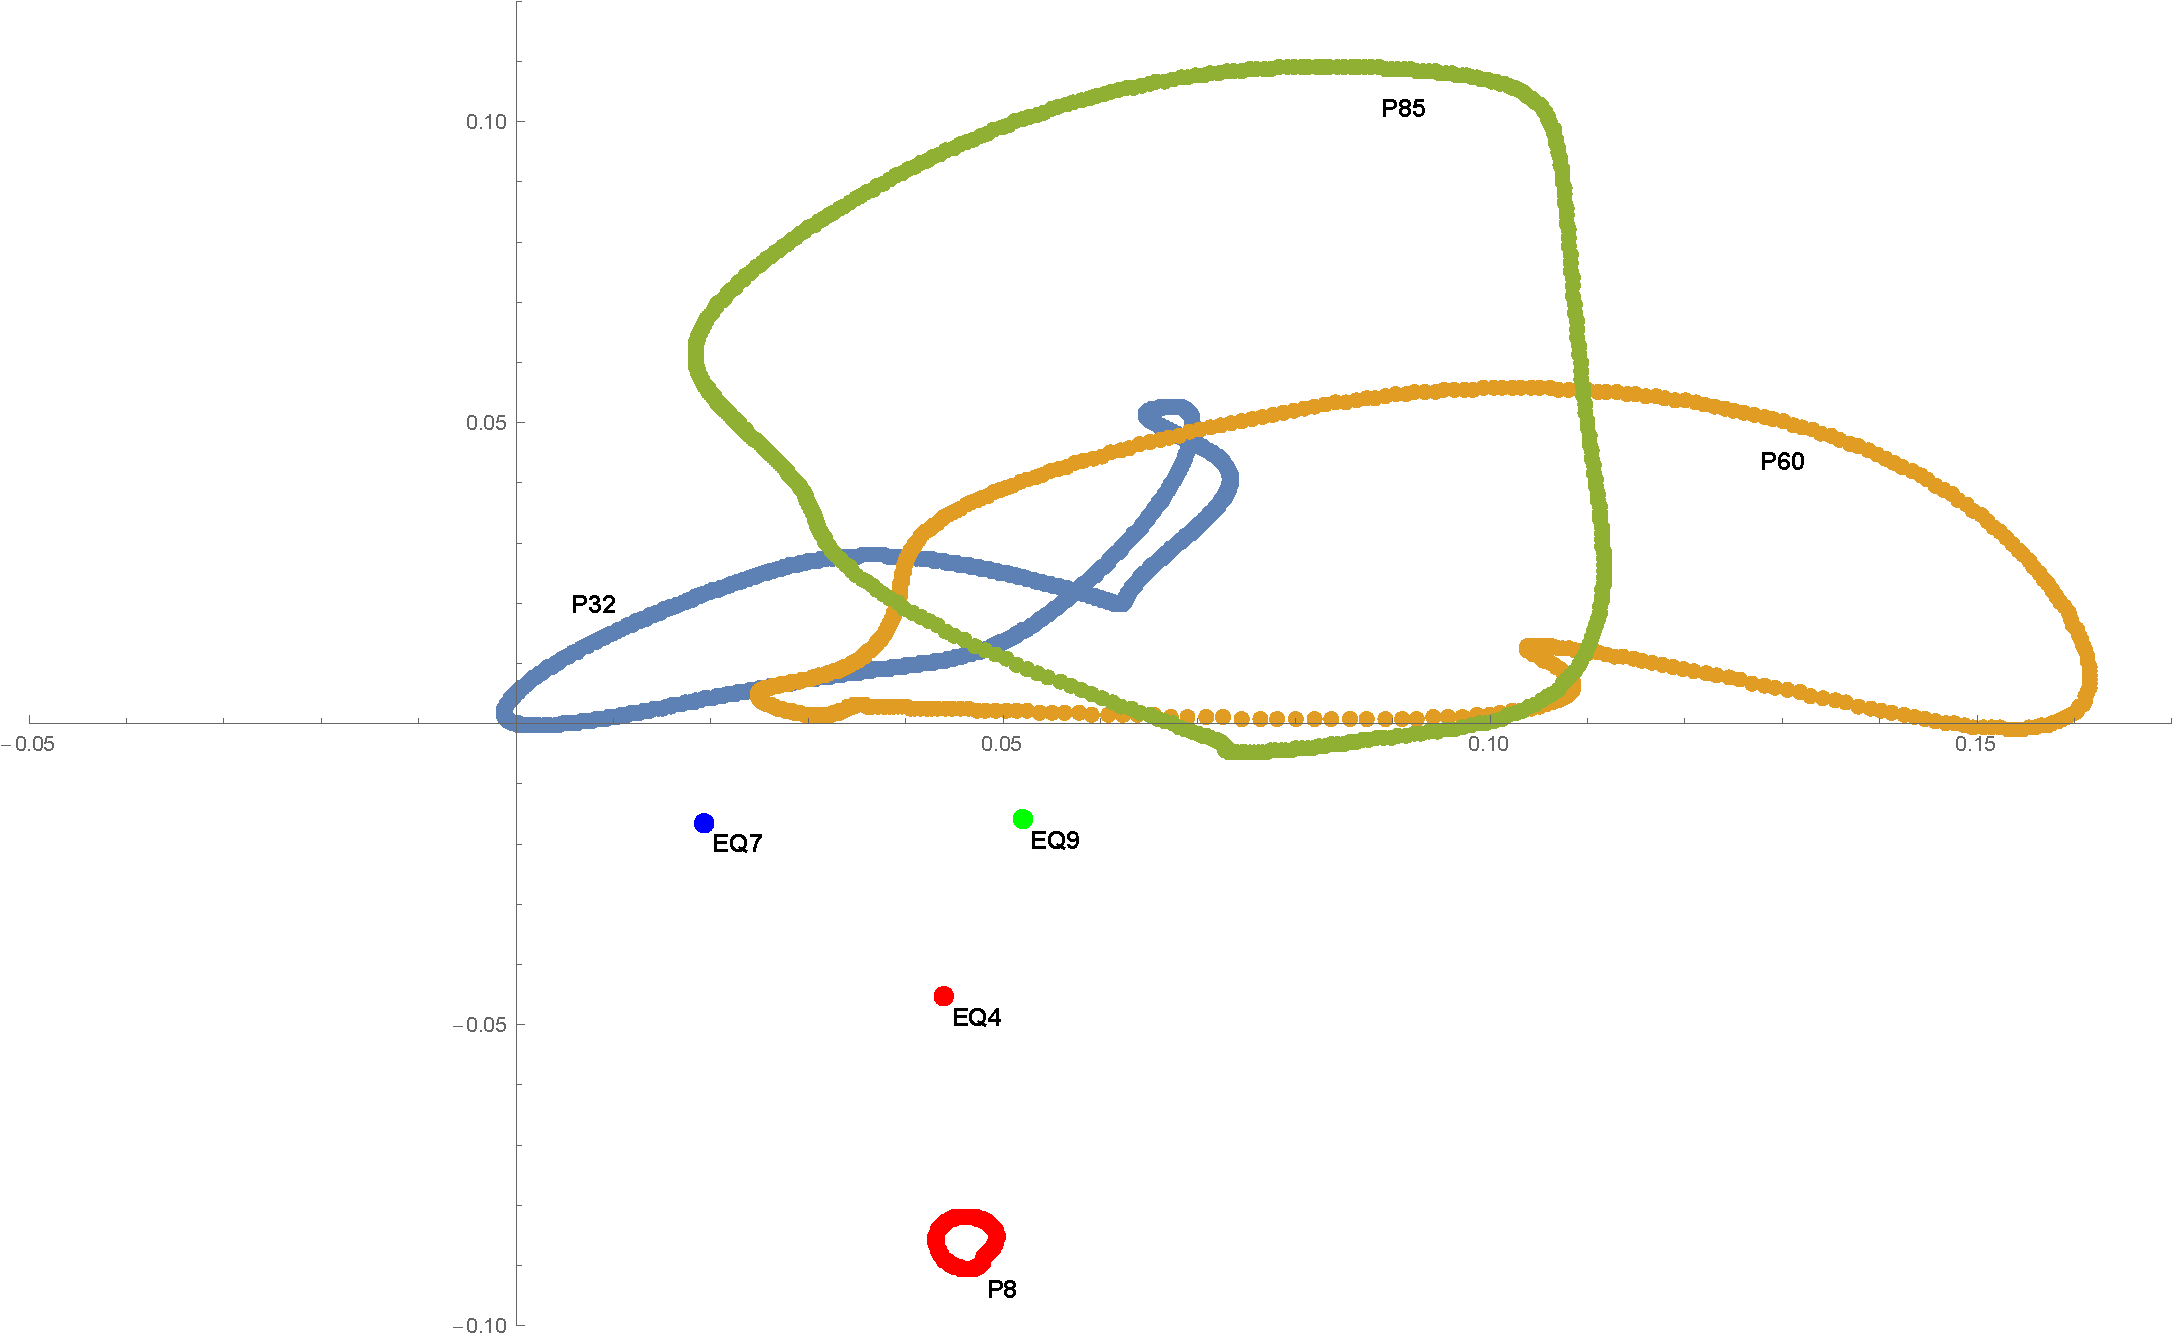
\includegraphics[width=\textwidth]{PeriodicOrbitPO412}
\caption{2D state space projection of the Gang of Four and some reference equilibria. The basis vectors for the projection were constructed by orthonormalizing the initial states of each of the periodic orbits. This results in a 4D state space projection, of which we can take 2D slices (of which there are 6), or 3D slices (of which there are 4). The equilibria are fully symmetric, and were found by Halcrow\rf{Halcrow2008}. Notice that the P8 orbit is separated by the equilibria from P85, P60 and P32, a feature that holds true in the other 5 2D projections.}\label{fig:POStateSpace}
\end{figure}

\subsubsection{State Space Projection}
If we have a set of $k$ basis vectors $\Vector{q}_i$ that are orthonormal and span a subspace $\mathfrak{V}_k \subset \mathfrak{V}$ of dimension $k$, then the projection of a vector $\Vector{v} \in \mathfrak{V}$ onto $\mathfrak{V}_k$ is defined 
\begin{equation}
\Vector{v}_k = \sum{i = 1}{k}{c_i \Vector{q}_i},
\end{equation}
where $c_i = \Vector{v} \cdot \Vector{q}_i$. When $k$ is either 2 or 3, we can visualize the $n$-dimensional trajectory as a 2 or 3 dimensional trajectory instead. While we lose information in making this projection, we can still gain a great deal of valuable information about trajectories. Projecting the four periodic orbits in \refFigRange{fig:p85}{fig:p8} onto a basis constructed from orthonormalizing the initial conditions of each orbit results in the state space projection in \refFig{fig:POStateSpace}.\\

 The main issue with the state space projection method, however, is that a state must be {\bf congruent} to a basis to be projected onto it - that is, both the box length and grid discretization must be the same for both the state and the projection basis. Many previous investigations\rf{Halcrow2008,Gibson2008} have important results in the W03 cell, where $(L_x,L_z) = (5.51157,2.51327)$, with corresponding state space projections. In order to compare to these results, we attempted to use \refAlg{alg:parCont} to continue the four periodic orbits into the W03 cell, which lead us to the next important result.

\section{Spanwise Continuation}

When \refAlg{alg:parCont} was used to continue P8 down to the W03 cell, the data presented in \refFig{fig:LZBif} was produced.  Initially, the continuation algorithm decreases $L_z$ and increases $T$, but at $L_z \approx 2.8$, the algorithm reverses itself, decreasing $T$ and increasing $L_z$, until $L_z \approx 2.95$, when the algorithm resumes decreasing $L_z$ and increasing $T$. Since we expect that the period of an orbit ought to uniquely define the orbit,\footnote{We generally assume that if two solutions have differing periods, they are distinct, which may seem reasonable - but holes in such a simple criterion are evident almost immediately. For example, two `distinct' orbits with periods $T_1$ and $T_2$ may in fact be the same orbit, with period $|T_2-T_1|$, that has simply repeated more times for one orbit than for the other. This hole can be plugged by any number of methods, most easiest by simply calculating $||\Vector{u}_1(t) - \Vector{u}_2||$ over the entire period. If the norm is never small, then the orbits are distinct. }  the existence of multiple, distinct orbits for $2.8 \leq L_z \leq 2.96$ hints at a bifurcation. 
\begin{figure}[t]
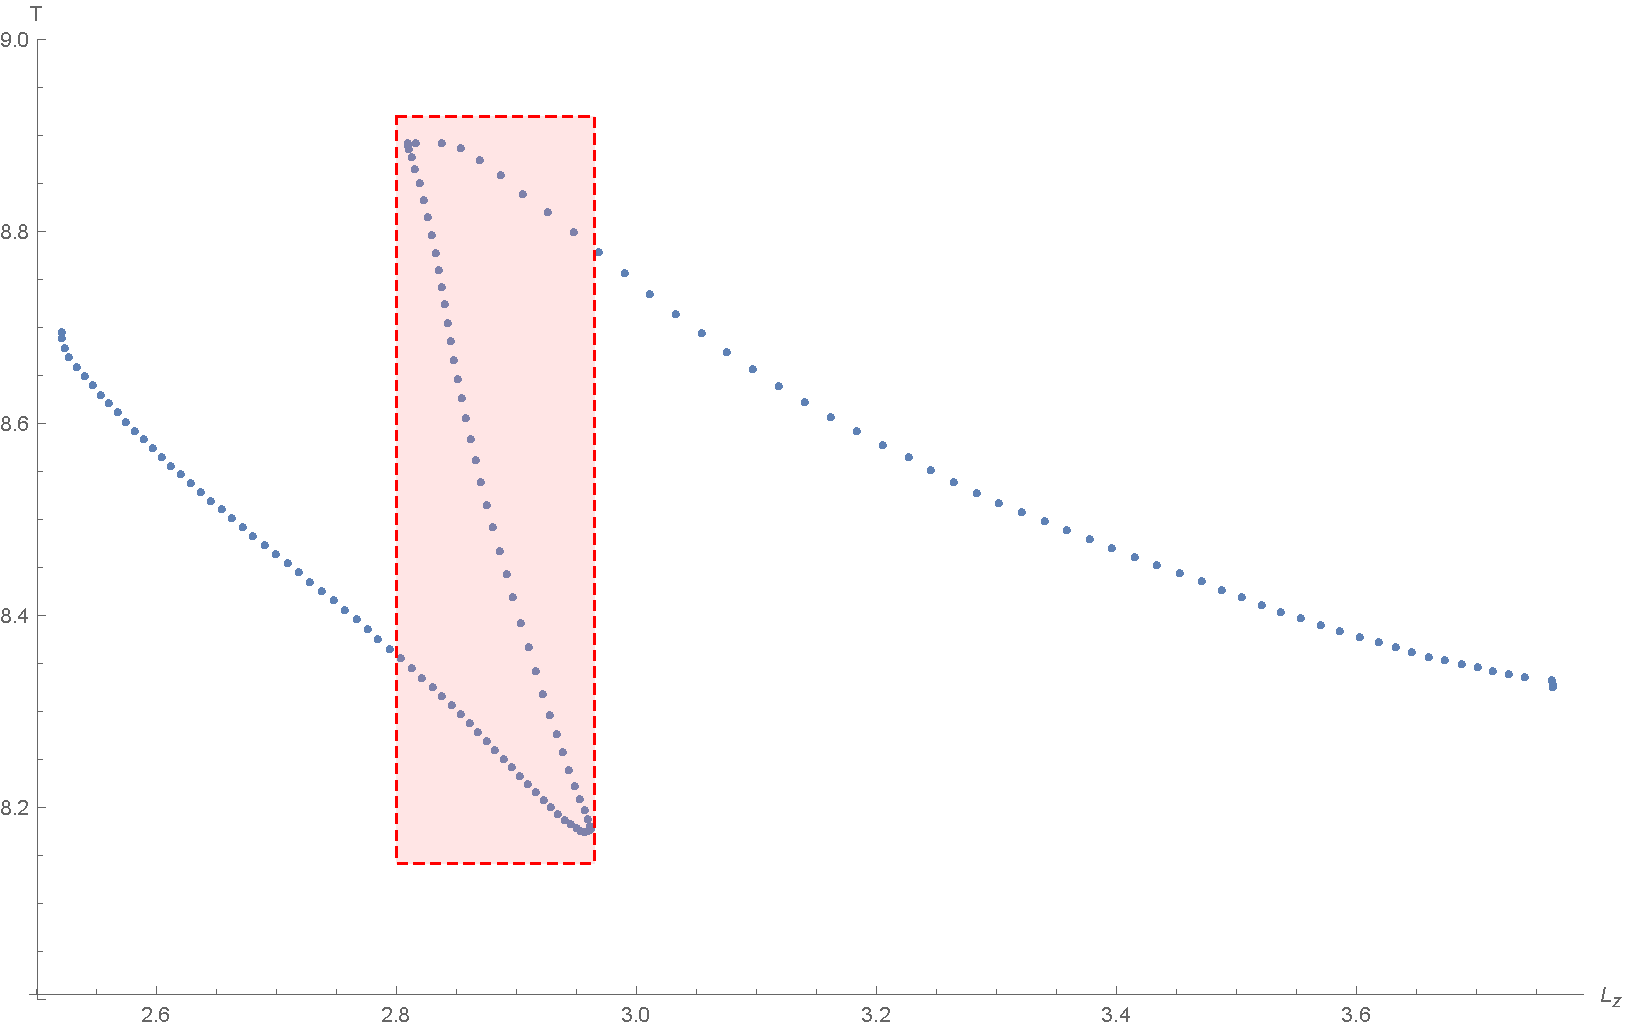
\includegraphics[width=\textwidth]{TLzBD}
\caption{Period as a function of spanwise cell length for P8. The data can be sectioned into three distinct parts. First, the {\bf upper branch} (blue circles), which is the path that the continuation algorithm initially follows in parameter space. Second, the {\bf transition branch} (green diamonds), which occurs after the {\bf first turning point} (red, dashed circle). Third, the {\bf lower branch} (orange rectangles), after the {\bf second turning point} (purple, solid circle). Within the marked rectangular region, multiple distinct solutions exist for the same cell length, hinting at a bifurcation. Searches at higher resolution have pinned down the turning points to the interval $L_z \in[2.8087, 2.8096]$ for the first turning point, and $L_z \in [2.6150,2.6157]$ for the second turning point.}\label{fig:LZBif}
\end{figure}
\begin{figure}[t]
\includegraphics[width=\textwidth]{phasePortraitTransition}
\caption{Phase portrait of the Van Der Pol oscillator and its Hopf bifurcation, with trajectories in white. (a), for negative values of the bifurcation parameter, the single periodic orbit is unstable, so an initial condition that begins near the orbit spirals away from it. (b), when the bifurcation parameter is zero, there is no periodic orbit. (c), for positive values of the bifurcation parameter, the periodic orbit is stable, and initial conditions are attracted into the orbit.}\label{fig:phasePortrait}
\end{figure}
 The similarity of \refFig{fig:LZBif} to \refFig{fig:bifurcations} is striking, and led us to suspect the possibility that P8 undergoes some form of bifurcation at $L_z \approx 2.8$ and $L_z \approx 2.95$. However, \refAlg{alg:parCont} relaxes the convergence criteria to $10^{-10}$ to speed up the parametric continuation process, and as a result, may have found artificial solutions, so we verified the existence of multiple distinct solutions for $L_z = 2.925$ and $(N_x,N_y,N_z) = (62,53,62)$ to $10^{-13}$. It is important to note that this in and of itself does not necessarily prove that a bifurcation exists -- for example, the continuation algorithm may have simply found \emph{another} periodic orbit's trajectory and hopped onto that. When a bifurcation occurs, the qualitative behavior of solutions pre and post-bifurcation tend to be markedly different. For low-dimensional systems, this is easy to evaluate, since one can visually identify changes in the phase space, as in \refFig{fig:phasePortrait}. For higher-dimensional systems, such an approach is not feasible. 

\subsection{Linear Stability Analysis}\label{sec:LSA}

We can instead turn to {\bf linear stability analysis}. If $\Vector{u}$ is a periodic orbit with period $T$, then for a small perturbation ${\bf \textrm{d}}\Vector{u}$, 
\begin{equation}\label{eq:linearStable}
 f_T(\Vector{u} + {\bf \textrm{d}}\Vector{u}) - \Vector{u} =  f_T(\Vector{u}) - \Vector{u} + \mathbb{J}_{T,\Vector{u}}{\bf \textrm{d}}\Vector{u} =  \mathbb{J}_{T,\Vector{u}}{\bf \textrm{d}}\Vector{u},
\end{equation} 
where $ \mathbb{J}_{T,\Vector{u}}$ is the Jacobian of the Navier-Stokes forward-time map evaluated at $\Vector{u}$. The stability of the orbit is determined by how  ${\bf \textrm{d}}\Vector{u}$ changes over time - if it shrinks, then the orbit is stable, but if it grows, it is unstable. Writing  ${\bf \textrm{d}}\Vector{u}$ as a linear combination of the eigenvectors $\Vector{v}_i$ of  $ \mathbb{J}_{T,\Vector{u}}$, the right-hand side of \eqref{eq:linearStable} becomes
\begin{equation}\label{eq:oneOrbit}
 \mathbb{J}_{T,\Vector{u}}{\bf \textrm{d}}\Vector{u} =  \mathbb{J}_{T,\Vector{u}}\sum{i = 1}{n}{c_i\Vector{v}_i} = \sum{i = 1}{n}{c_i\lambda_i\Vector{v}_i},
\end{equation}  
where the $\lambda_i$ are the corresponding eigenvalues, known as the {\bf Floquet exponents}, whose real parts measure the exponential rate of decay or growth of the corresponding eigenvector.\footnote{The real parts are known as the {\bf Lyapunov exponents}. The imaginary part contributes only to the oscillatory behavior.}   From this definition, it is clear that the periodic orbit can only be stable against infinitesimal perturbations if $\textrm{Re}[\lambda_i]  \leq 0~\forall~i$, and unstable otherwise. The eigenvalues for the Navier-Stokes forward-time map can be calculated by \refAlg{alg:Arnoldi}. The eigenvalues of P8 in the HKW cell at $\ReN=400$ are shown in \refFig{fig:P8Eigenvals}

\begin{figure}[h]
\includegraphics[width=\textwidth]{P8Eigenvals}
\caption{All 20 unstable eigenvalues, and the 80 largest stable or marginal $(|\lambda| << 1)$ eigenvalues of P8, in the HKW cell at $\ReN=400$. Note that the eigenvalues come in conjugate pairs. Since there are eigenvalues with positive real parts, the periodic orbit is unstable, as expected. Note that since the Jacobian likely has full rank, and likely also has no repeating nonzero eigenvalues, there are several orders of magnitude more stable eigenvalues than there are unstable. Since the Arnoldi iteration will find the larger eigenvalues first, all the unstable eigenvalues are shown, whereas only the weakly stable eigenvalues are calculated.}\label{fig:P8Eigenvals}
\end{figure}

In general, we would expect that as the control parameter changes, the Lyapunov exponents would also. In particular, if a change in the control parameter resulted in the Lyapunov exponent changing sign, the qualitative behavior of the periodic orbit would change, resulting in a bifurcation. Applying the Arnoldi iteration to the states near the turning points of \refFig{fig:LZBif} results in \refFig{fig:P8FirstBifurcation} and \refFig{fig:P8SecondBifurcation}. 
\clearpage
 \refFigs{fig:P8FirstBifurcation}{fig:P8SecondBifurcation} have a set of eigenvalues that switch sign at $L_z$ values that are reasonably consistent with turning point data from \refFig{fig:LZBif}. It therefore seems likely that these turning points do in fact correspond to bifurcations. Qualitative differences between the upper and transition branch are also apparent from observations of movies of the periodic orbit.\footnote{Available at {\tt https://youtu.be/JDzQfjx5Cmg}} From the video, it appears that the upper branch has more energy concentrated in the streaks than the transition branch, which in turn appears to have more energy in the mid-plane. \\

\begin{figure}[t]
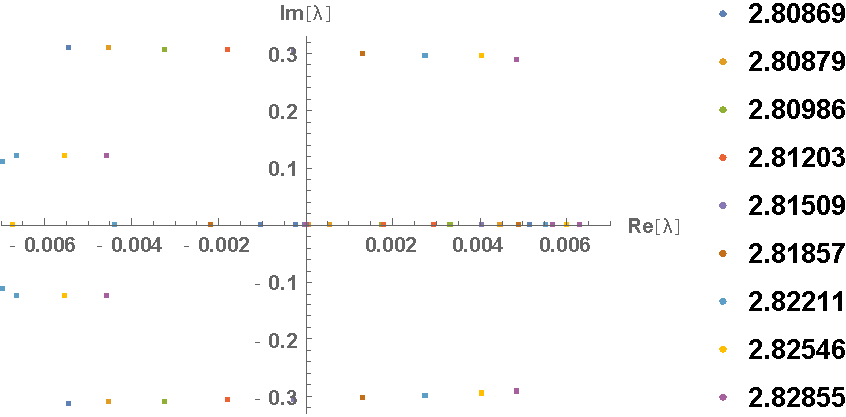
\includegraphics[width=\textwidth]{P8FirstBifurcation}
\caption{Eigenvalues of P8 as a function of $L_z$ at the first turning point. When the real part of the eigenvalue switches sign, the associated eigenvector switches stability. Therefore, the line of eigenvalues with imaginary part  $\approx \pm 0.3$ are of special interest.  The real part of the eigenvalue likely switches sign at some $L_z \in [2.81509,2.81857]$, compared to the first turning point, which likely occurs for $L_z \in [2.8087205, 2.8096095]$  }\label{fig:P8FirstBifurcation}
\end{figure}


\begin{figure}[h]
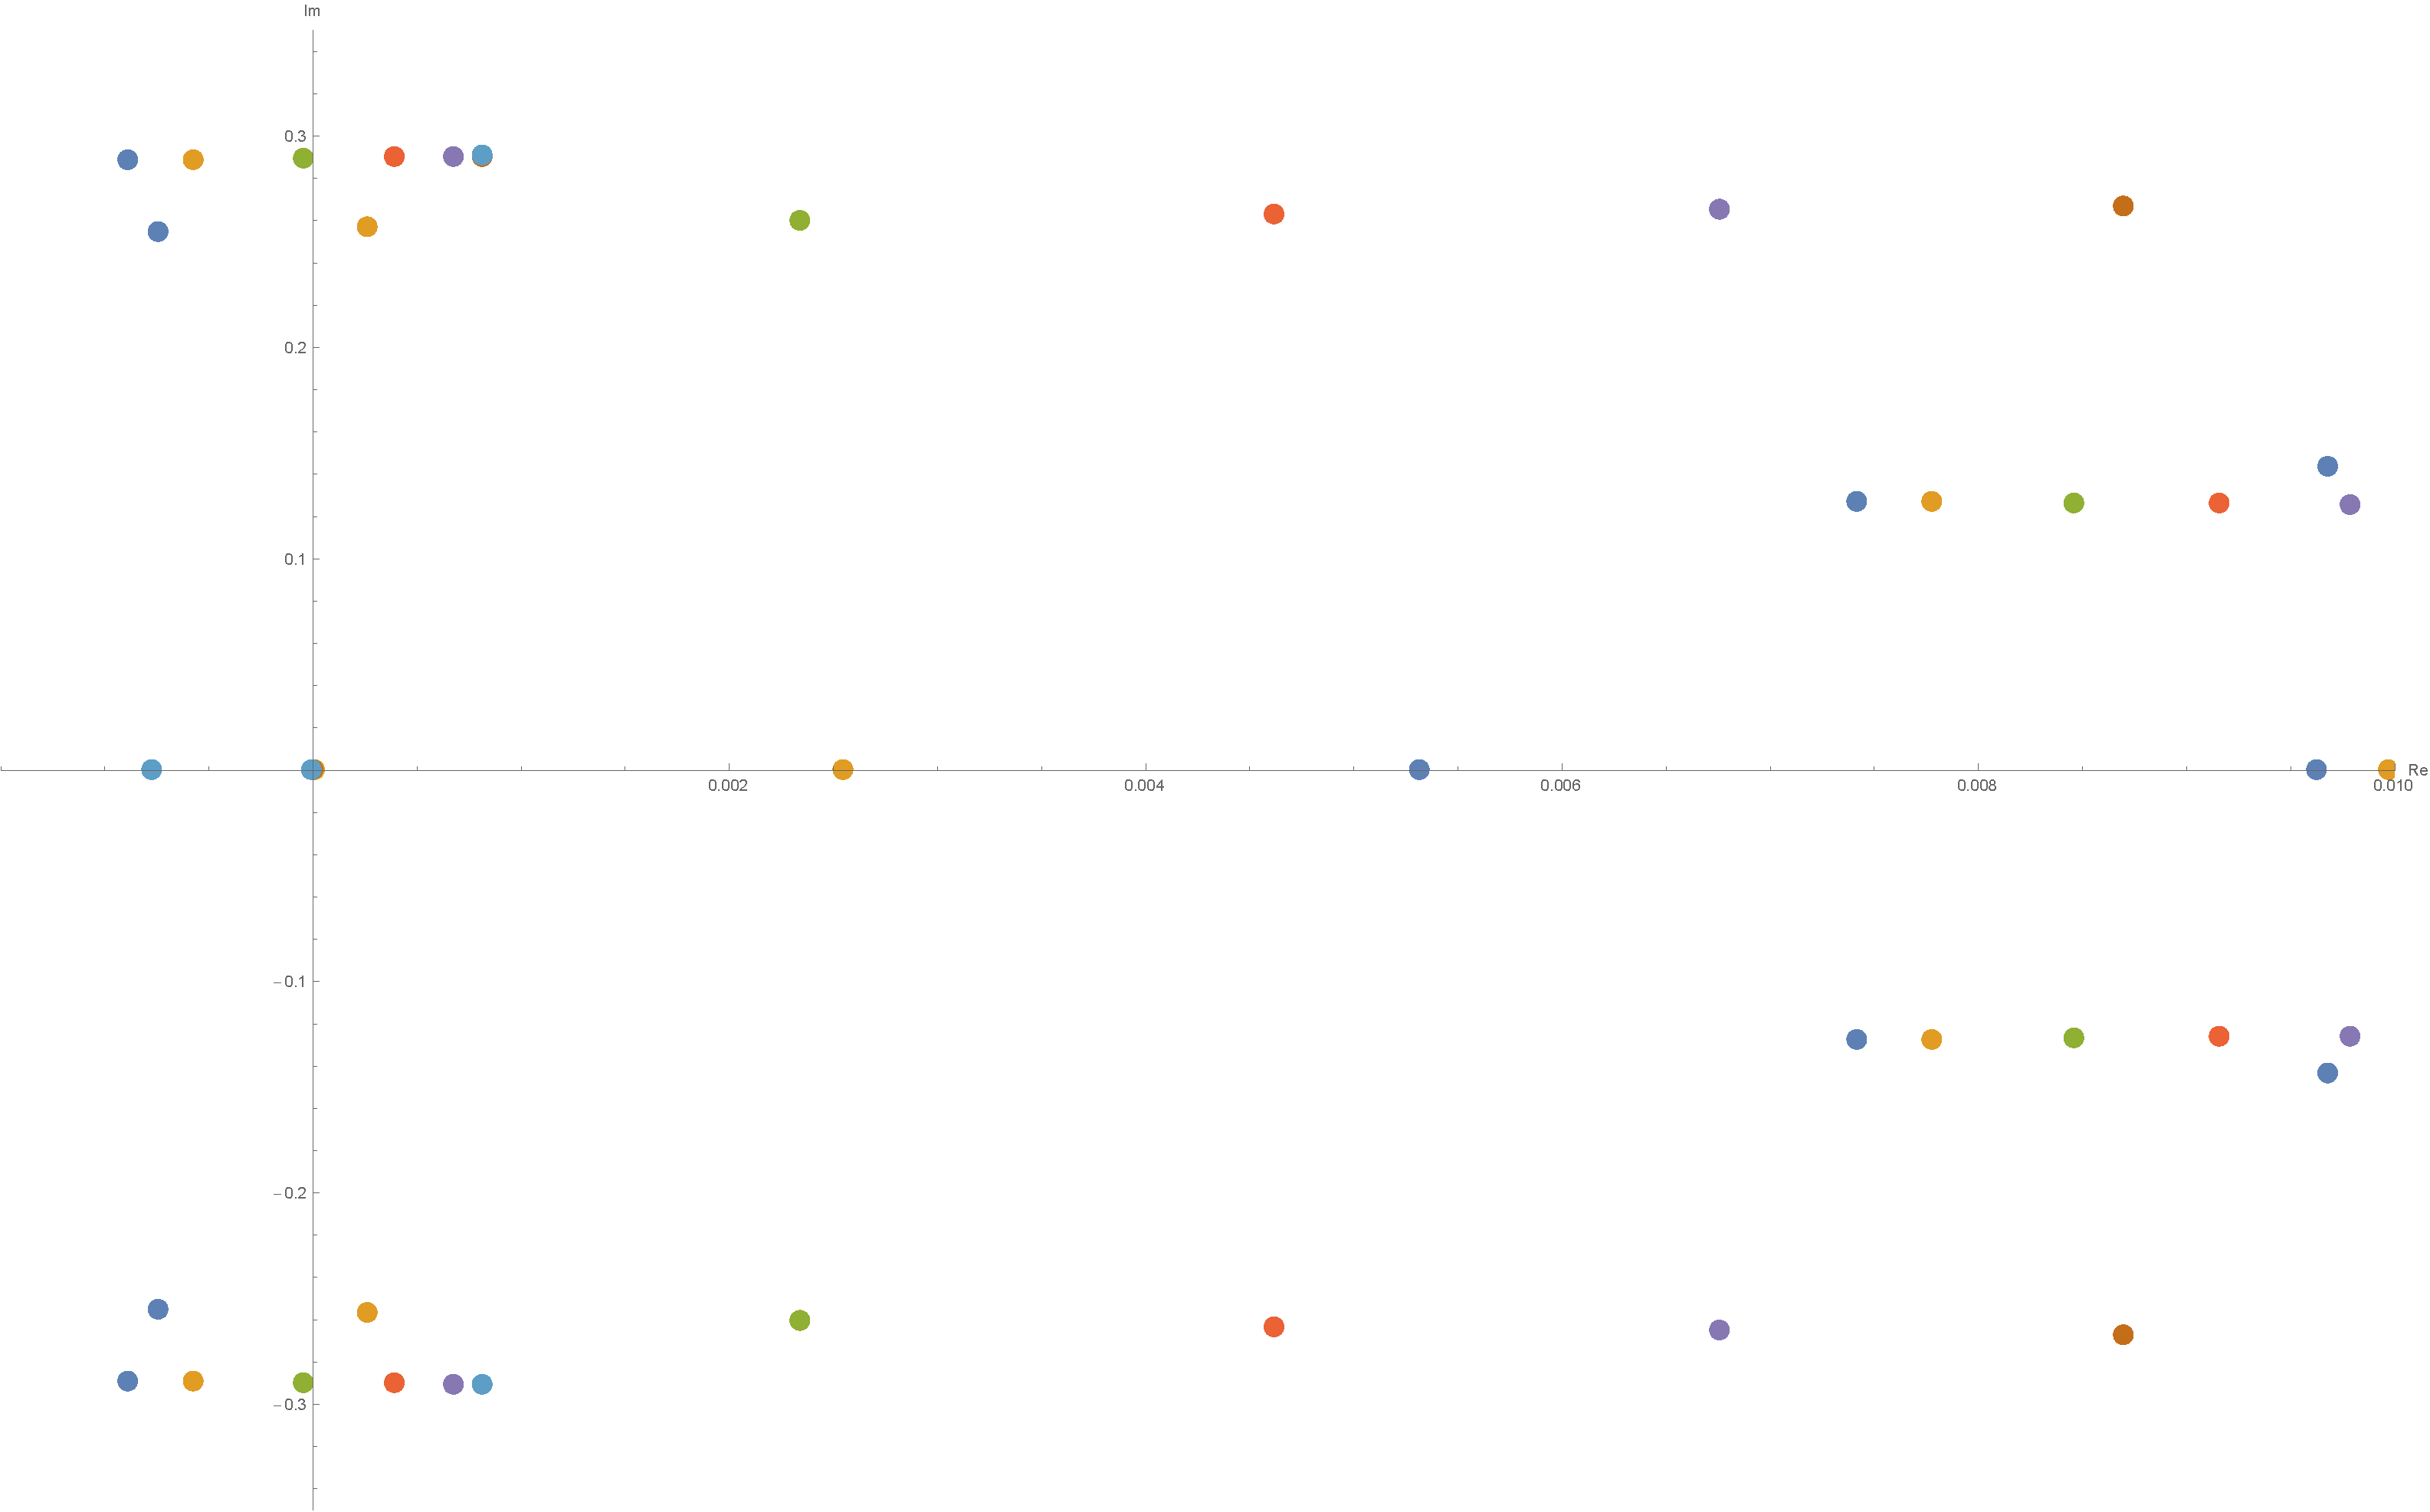
\includegraphics[width=\textwidth]{P8SecondBifurcation}
\caption{Eigenvalues of P8 as a function of $L_z$ at the second turning point. Here, two sets of eigenvalues have real parts that switch signs, first in the invertval $L_z \in [2.96122,2.96137]$ and second in the interval $L_z \in [ 2.96142,2.9615]$. The second stability switch is consistent with the position of the second turning point, which occurs in the interval $L_z \in [2.6150,2.6157]$.}\label{fig:P8SecondBifurcation}
\end{figure}

\subsection{Return of the State Space}

Having used linear stability analysis to find the unstable eigenvector, we can use the state space projection to visualize the effect of a slight perturbation, as  in \refFig{fig:p8E1}. Here, we see the effect of a slight perturbation along the most unstable eigenvector $P8E1$, with eigenvalue $0.0998 - 0.2605 i$. Now \refFig{fig:p8E1} is noisy, and difficult to analyze. To deal with this, we can construct the {\bf Poincare section} of a trajectory. The Poincaré section of a $k$ dimensional trajectory is constructed by keeping track of where the trajectory crosses a $k-1$ dimensional surface. The Poincare section for  $P8E1$, displayed in \refFig{fig:E1Poincare} displays the qualitative behavior we would expect for a complex eigenvalue - the real part is negative and the perturbation grows, the imaginary part is nonzero, and the perturbation spirals around the initial position. Even though the eigenvalue is only valid locally, we can still see that it approximately predicts the behavior of the trajectory - from the imaginary part of the eigenvalue, we can see that it ought to take approximately 25 time units for a full rotation in the Poincare section. \refFig{fig:E1Poincare} suggests that approximately 5 orbits have taken place for a full rotation in the Poincare section, each with periods that are approximately 8 time units. This does not agree exactly,\footnote{Or very well at all, especially since we've just come from having residuals on the order of $10^{-14}$} but one must remember that the Floquet exponents are a \emph{local} model of the orbit, and naturally become less precise the more the perturbation grows.\footnote{As a matter of fact, the pictured spiral is the last spiral the Poincare section trajectory executes, though the trajectory in the full space continues to look qualitatively similar to the original orbit for a long time.}   


\begin{figure}[h!]
\centerline{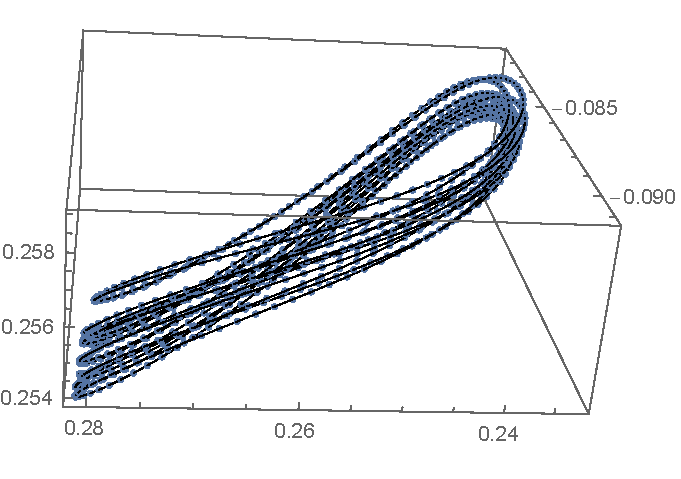
\includegraphics[scale=1]{E1Perturb}}
\caption{The trajectory of a slight perturbation along the most unstable eigenvector, projected onto a difference slice of the same basis as in \refFig{fig:POStateSpace}. Notice that it keeps the general shape of the orbit that spawned it, at least for short time spans.}\label{fig:p8E1}
\end{figure}

\begin{figure}[h!]
\centerline{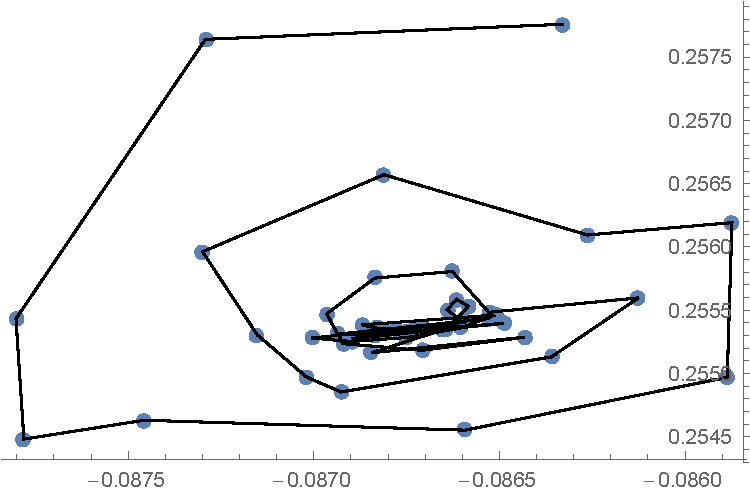
\includegraphics[scale = 0.9]{E1Poincare}}
\caption{Poincaré section of \refFig{fig:p8E1}, defined by the surface $e_2 = 0.26$. Notice that the trajectory along the Poincare section spirals outwards, as we would expect for an unstable manifold with a complex eigenvalue.}\label{fig:E1Poincare}
\end{figure}

\section{Dissipation and Energy Input} 
  
\subsection{A New Projection}
While \refFig{fig:POStateSpace} seems to indicate that P8 is a special member of the Gang of Four -- an assertion which is backed up by the marked difference in the properties displayed in \refTab{tab:summary} -- the striking dissimilarity in \refFig{fig:POStateSpace} may be an artifact of the projection basis. To address this issue, we can also project onto the {\bf dissipation-energy input} (DI) plane, where the dissipation $D$ and energy input $I$ are defined
\begin{align}
D(t) = \frac{1}{L_xL_yL_z}\int{0}{L_x}{\int{0}{L_y}{\int{0}{L_z}{|\nabla\times\Vector{u}(t)|^2}{\textrm{d}z}}{\textrm{d}y}}{\textrm{d}x},\label{eq:diss}\\
I(t)  = 1 + \frac{1}{2L_xL_z}\int{0}{L_x}{\int{0}{L_z}{\pder{1}{\Vector{u}_{y}}{y} |_{y=1}+\pder{1}{\Vector{u}_{y}}{y} |_{y=-1}}{\textrm{d}z}}{\textrm{d}x}.\label{eq:einp}
\end{align} 
Unlike the state space projection, which is to some extent an artificial projection mechanism, the DI plane projection has real physical meaning, and thus is a more natural projection. Applying \refeqs{eq:diss}{eq:einp} to the Gang of Four results in \refFig{fig:DIGOF},\footnote{Note that for a periodic orbit, the mean dissipation and energy input need to be balanced, which explains why all observed solutions do not stray far away from the line $D(I) = I$.} which suggests that the distinctive features of P8 are likely not artificial. However, a glance at \refFig{fig:turbDI}, which overlays random turbulent trajectories on \refFig{fig:DIGOF} suggests that P8 is the only member of the Gang of Four that does not seem to directly influence turbulent trajectories in any significant way, and that P85 may have a significant influence instead. However, since the Arnoldi iteration scales linearly with the period, analysis of any of the longer orbits would take an unfeasibly long time with our computing resources. As a result, we will limit our analysis to P8.\footnote{For example, a single iteration of \refAlg{alg:parCont} takes about 2 hours for P8, which allowed us to collect the data presented in \refFig{fig:LZBif} in about a week. The same process would have taken more than a month for P32, and several for P60 and P85.}   
\begin{figure}[h]
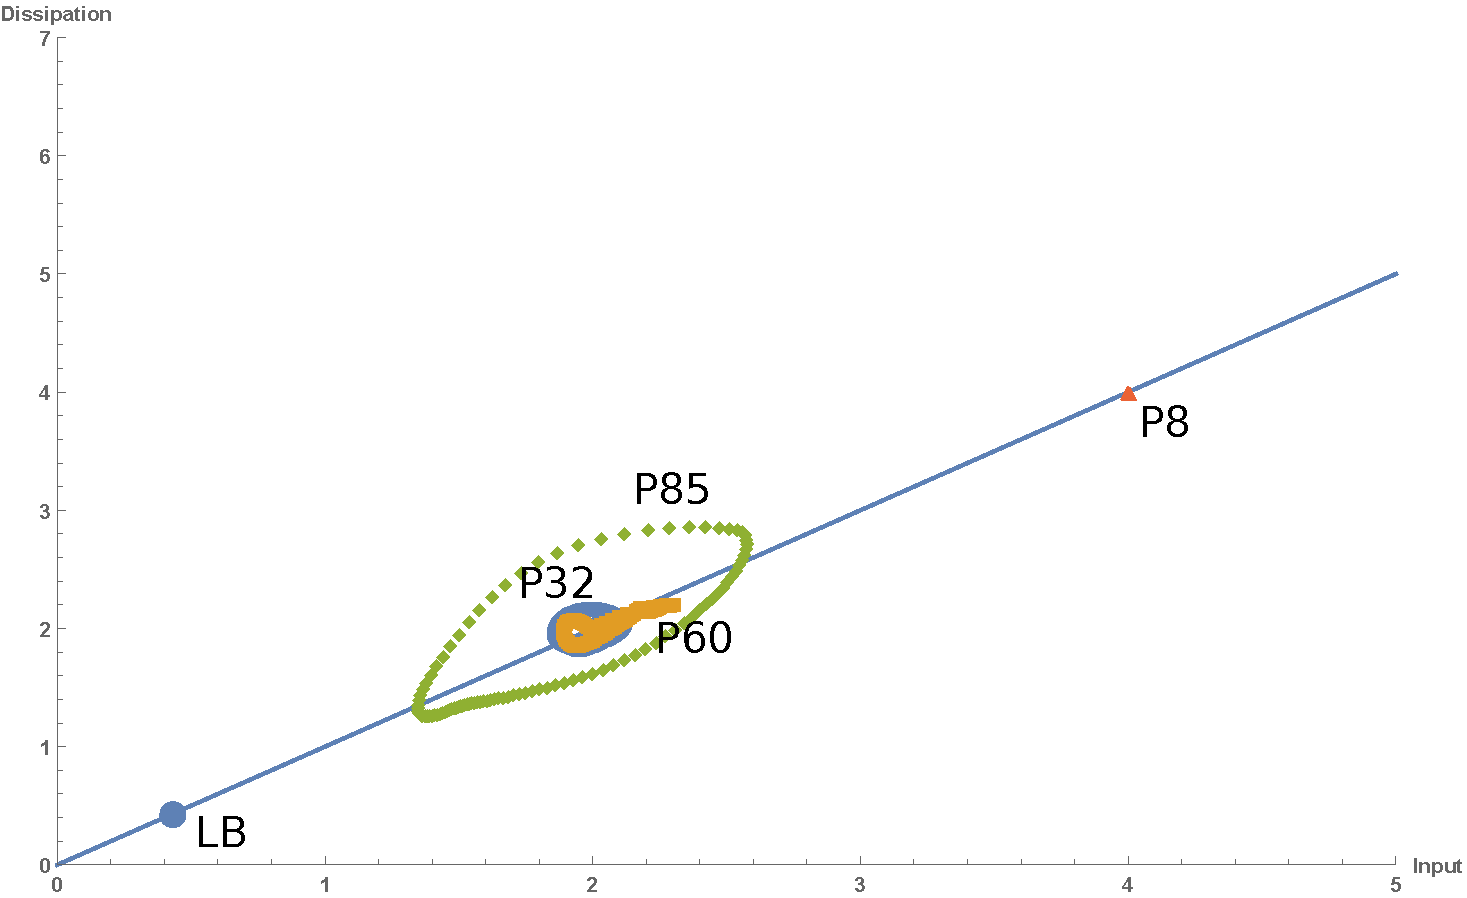
\includegraphics[width=\textwidth]{DIOG}
\caption{DI projection of the Gang of Four, the Nagata lower branch equilibirum (LB), and the line of equal dissipation-energy input. While the lesser members of the Gang remain clustered towards a input/dissipation of 2, P8 stays at near dissipation/input of 4. Due to P8's low period, the fine details of its orbit cannot be discerned here. The separation observed in \refFig{fig:POStateSpace} is clearly reflected in this physically important projection.}\label{fig:DIGOF}
\end{figure}

\begin{figure}[h]
\includegraphics[width=\textwidth]{DearGodWhy}
\caption{DI plane projection of 20 turbulent trajectories (red and blue) beginning from random initial conditions, with perturbations of magnitude $0.3$ overlaid on the Gang of Four, the Nagata upper branch equilibrium, and the line of equal dissipation-energy input. The data implies that P8 contributes very little to the dynamics of turbulence, since turbulent trajectories do not appear to `live' near P8. It does, however, suggest that P85 may have some importance in turbulent transition, since the trajectories only remain `bound' to a narrow area of D-I space while they are within the orbit of P85.}\label{fig:turbDI}
\end{figure}

\subsection{The Search for Bifurcations, Part II}
The DI projection has another extremely important benefit -- it is domain-agnostic. This allows us to compare the different branches of \refFig{fig:LZBif} in a more sophisticated manner. Since the full bifurcation diagram spans a vast distance in the dissipation-energy input plane, the projection is divided into three parts, with te upper branch in \refFig{fig:DIUpper}, the transition branch in \refFig{fig:DITrans} and the lower branch in \refFig{fig:DILower}, where the divisions between branches is informed by \refFig{fig:LZBif}. Unfortunately, apart from the expected repulsion of the upper branch from the high dissipation/energy input zone, nothing particularly interesting occurs here.\\


\begin{figure}[h]
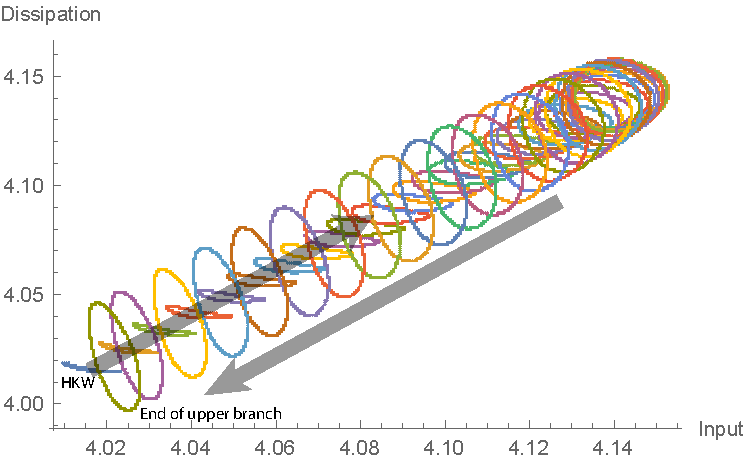
\includegraphics[width=\textwidth]{DIUpper}
\caption{DI plane projection of the upper branch of P8. The HKW solution is the thin blue solution that is continued up to higher dissipation/energy input. However, for finite \ReN, there is a maximum velocity gradient that can be maintained, so the energy input is necessarily bounded, and the orbits begin moving down the dissipation/energy input line, eventually becoming the transition branch. While we were hoping to see an especially meaningful change in the orbit topology, there doesn't seem to be a great deal of change in its general structure during any bifurcation. }\label{fig:DIUpper}
\end{figure}

\begin{figure}[h]
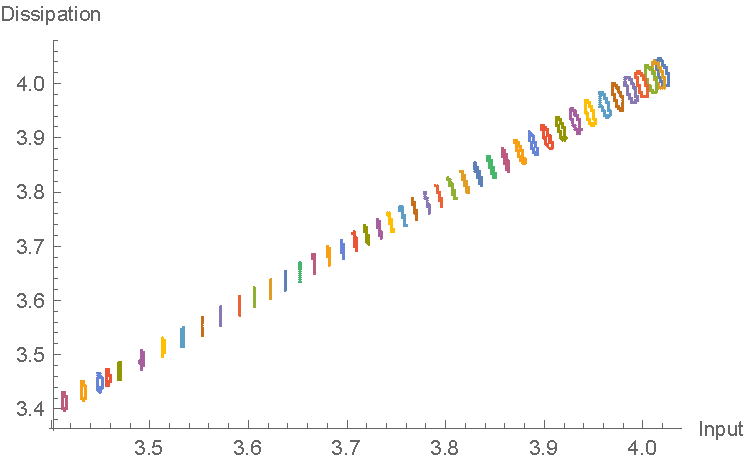
\includegraphics[width=\textwidth]{DITrans}
\caption{The transition branch continues to move down the dissipation/energy input line. As it does so, its area contracts to a near point, and expands again, at which point it becomes the lower branch. }\label{fig:DITrans}
\end{figure}

\begin{figure}[h]
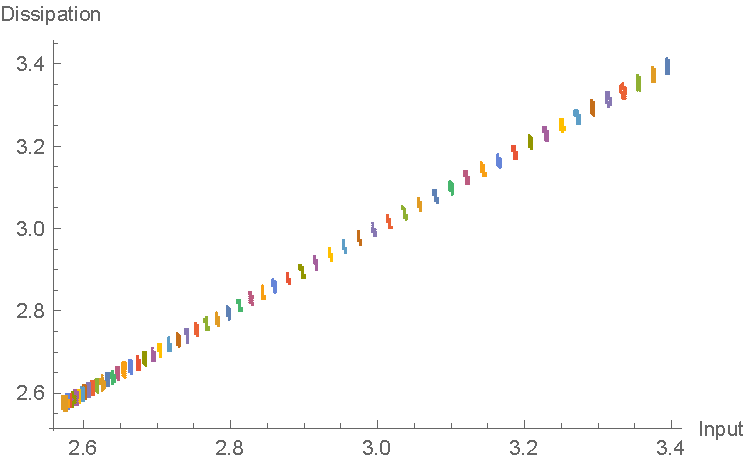
\includegraphics[width=\textwidth]{DILower}
\caption{The lower branch is even less eventful than the transition branch, and generally mantains its structure through its descent towards the origin of the DI plane. Eventually, it reaches the point where \refAlg{alg:parCont} fails, and the continuation process halts.}\label{fig:DILower}
\end{figure}

However, a glance at \refFigss{fig:DIUpper}{fig:DITrans}{fig:DILower} indicates that they are by and large elliptical in shape, so the area enclosed by the orbit can easily be calculated by the singular value decomposition. Applying this method and ordering by traversal down the continuation trajectory gives \refFig{fig:areaOrder}, whereas ordering by $L_z$ gives \refFig{fig:areaCell}. The results of this analysis are promising, since they show structural changes in a physically important projection, which occur near the expected location of the turning points. We can also easily calculate the circumference of each orbit by summing the distance between each individual point over the orbit, and obtain \refFig{fig:circumCell}, which is suggestively similar to \refFig{fig:LZBif}. \\

\begin{figure}[h!]
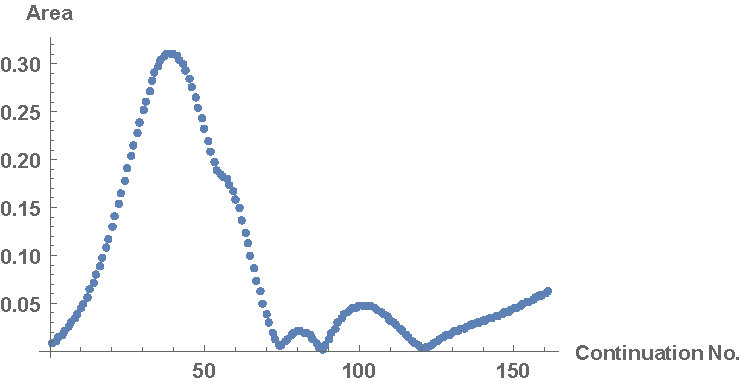
\includegraphics[width=\textwidth]{areaOrder}
\caption{Approximate area of P8 at various $L_z$. Here, the orbits are ordered by traversing \refFig{fig:LZBif}, beginning from the start of the upper branch. The area function begins looking very smooth and Gaussian, but acquires a kink on its way down, after which it behaves in a more complex manner. The fact that the area in the DI plane goes very low is interesting, but probably not indicative of any behavior that has a global effect.}\label{fig:areaOrder}
\end{figure}

\begin{figure}[h!]
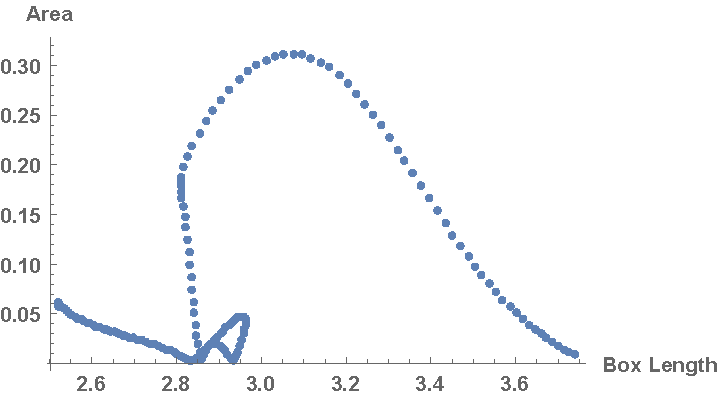
\includegraphics[width=\textwidth]{areaCell}
\caption{When the approximate area of P8 is ordered by $L_z$, the features observed in \refFig{fig:areaOrder} take on more meaning. The kink observed in the downwards slope of the Gaussian coincides almost perfectly with the first turning point of \refFig{fig:LZBif}, and the third peak corresponds to the second turning point. While not conclusive, this does show that the turning points are associated with (admittedly slight) structural changes in a physically important projection. }\label{fig:areaCell}
\end{figure}

\begin{figure}[h!]
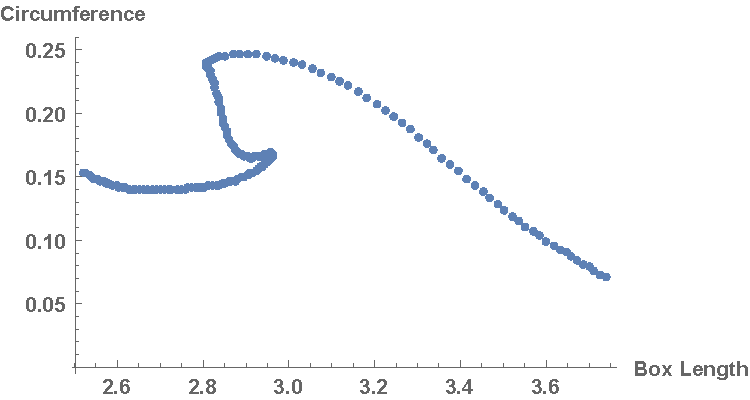
\includegraphics[width=\textwidth]{circumCell}
\caption{The circumference of P8 as a function of $L_z$. The similarly to \refFig{fig:LZBif} is noticeable, and is not as trivial as it may sound - the velocity on a trajectory is not certain \emph{a priori}, so a periodic orbit with a small circumference can still have a long period.}\label{fig:circumCell}
\end{figure}

\clearpage 
This ends the analysis of the Gang of Four, and of P8 in particular (Though not for lack of material to analyze...). We will now conclude this thesis by giving a quick summary of the key points, discussing the results, and suggesting potential areas of future research. 

	\chapter*{Conclusion}
         \addcontentsline{toc}{chapter}{Conclusion}
	\chaptermark{Conclusion}
	\markboth{Conclusion}{Conclusion}
	\setcounter{chapter}{5}
	\setcounter{section}{0}
	\epigraph{
	Well-chosen, non-frivolous epigraphs can enhance a thesis.
	}{Michael Scott} 

\section{Summary}

The goal of this thesis has been to find and investigate numerically the properties of \ecs\ with broken symmetry. The hope was that these symmetry broken \ecs\ would better predict  turbulent dynamics, which itself has no symmetry at all. As a result, understanding symmetry broken \ecs\ may lead to a more fundamental understanding of turbulent dynamics. Four periodic orbits, nicknamed the Gang of Four, were found, with periods ranging from 8 to 85 time units, in fully and partially symmetric subspaces. The symmetric periodic orbits (P85 and P60) have no relative velocity and a low number of unstable eigenvectors. On the other hand, the asymmetric periodic orbits (P32 and P8) have some streamwise and spanwise relative velocity respectively, consistent with their broken streamwise and spanwise symmetry (\refTab{tab:summary}).  Projection of the Gang of Four onto the dissipation-energy input plane in \refFig{fig:turbDI} indicates that P8 likely has no influence on turbulent dynamics. However, as computational resources are limited and the cost of analysis scales linearly with the period, we were forced to choose P8 as the principle orbit of investigation. \\ 

Application of the Arnoldi iteration gave the unstable eigenvalues and corresponding eigenvectors of P8. Perturbing P8 along the most unstable eigenvector gives the trajectory in \refFig{fig:p8E1}. Computing its Poincare section gives the spiral structure seen in \refFig{fig:E1Poincare}, which is relatively consistent with theoretical behavior. Parametric continuation of P8 in the spanwise box length $L_Z$ results in behavior suggestive of a bifurcation, with two turning points at which the continuation algorithm switches from reducing $L_z$ and increasing $T$ to increasing $L_z$ and reducing $T$ and vice versa, shown in the S-shaped diagram in \refFig{fig:LZBif}. Analysis of the eigenvalues at both sides of the turning points (\refFigs{fig:P8FirstBifurcation}{fig:P8SecondBifurcation}) suggested that a manifold changed stability (from stable to unstable) in both cases, at a location that was consistent with the turning point.  In addition, fitting the DI projection of P8 at various box lengths both to the area and circumference of the orbit gave relations that show changes in its behavior at $L_z$ consistent with the turning points (\refFigs{fig:areaCell}{fig:circumCell}). Given the consistently strong indicators that significant structural changes occur, it seems reasonable to conclude that there is some local change in the state space that is consistent with the occurence of a bifurcation at the turning points $\mathfrak{Z}_1$ and $\mathfrak{Z}_2$.\\


\section{Future Work}

There are many threads of investigation we would have liked to have followed up on, time permitting. Most importantly, we would have investigated in more detail the behavior of the neglected members of the Gang of Four, which may have led in directions that we cannot anticipate. As far as P8 is concerned, preliminary data suggests that fully symmetric periodic orbits have a larger proportion of purely real unstable eigenvectors in comparison to partially symmetric periodic orbits. Since the behavior of a perturbation along a complex eigenvector would likely lead to more complex, chaotic behavior, it may be possible that trajectories near partially-symmetric orbits have, for instance, enhanced mixing properties when compared to trajectories near fully symmetric orbits. We would have also liked to have parametrically continued P8 in \ReN, since physical intuition suggests that it ought to appear from a bifurcation at some critical $\ReN < 400$.  It was also noted that when P8 was discovered from a guess generated by a random perturbation off of P60, the trajectory fell into its temporary orbit around P8 extremely quickly, despite the fact that P60 and P8 appear to live in distinct parts of the phase space of \refFigs{fig:POStateSpace}{fig:DIGOF}, and trajectories originating from near P60 in the DI projection appear to all move \emph{away} from P8. One possible explanation for this is that there exists some heteroclinic connection between P8 and P60 that guided the perturbation.  
	%\chapter{Tables and Graphics}

\section{Tables}
	The following section contains examples of tables, most of which have been commented out for brevity. (They will show up in the .tex document in red, but not at all in the .pdf). For more help in constructing a table (or anything else in this document), please see the LaTeX pages on the CUS site. 

\begin{table}[htdp] % begins the table floating environment. This enables LaTeX to fit the table where it works best and lets you add a caption.
\caption[Basic Table 1]{A Basic Table: Correlation of Factors between Parents and Child, Showing Inheritance} 
% The words in square brackets of the caption command end up in the Table of Tables. The words in curly braces are the caption directly over the table.
\begin{center} 
% makes the table centered
\begin{tabular}{c c c c} 
% the tabular environment is used to make the table itself. The {c c c c} specify that the table will have four columns and they will all be center-aligned. You can make the cell contents left aligned by replacing the Cs with Ls or right aligned by using Rs instead. Add more letters for more columns, and pipes (the vertical line above the backslash) for vertical lines. Another useful type of column is the p{width} column, which forces text to wrap within whatever width you specify e.g. p{1in}. Text will wrap badly in narrow columns though, so beware.
\toprule % a horizontal line, slightly thicker than \hline, depends on the booktabs package
  Factors &  Correlation between Parents \& Child & Inherited \\ % the first row of the table. Separate columns with ampersands and end the line with two backslashes. An environment begun in one cell will not carry over to adjacent rows.
  \midrule % another horizontal line
Education & -0.49 & Yes \\ % another row
Socio-Economic Status & 0.28 & Slight \\
Income & 0.08 & No\\
Family Size & 0.19 & Slight \\
Occupational Prestige &0.21 & Slight \\
\bottomrule % yet another horizontal line
\end{tabular}
\end{center}
\label{inheritance} % labels are useful when you have more than one table or figure in your document. See our online documentation for more on this.
\end{table}

	\clearpage 
%% \clearpage ends the page, and also dumps out all floats. 
%% Floats are things like tables and figures.

If you want to make a table that is longer than a page, you will want to use the longtable environment. Uncomment the table below to see an example, or see our online documentation.

	\begin{longtable}{||c|c|c|c||}
	 	\caption[Long Table]{An example of a long table, with headers that repeat on each subsequent page: Results from the summers of 1998 and 1999 work at Reed College done
by Grace Brannigan, Robert Holiday and Lien Ngo in 1998 and Kate Brown and
Christina Inman in 1999.}\\ \hline
	    	  \multicolumn{4}{||c||}{Chromium Hexacarbonyl} \\\hline
		   State & Laser wavelength & Buffer gas & Ratio of $\frac{\textrm{Intensity
at vapor pressure}}{\textrm{Intensity at 240 Torr}}$ \\ \hline
		  \endfirsthead
		\hline     State & Laser wavelength & Buffer gas & Ratio of
$\frac{\textrm{Intensity at vapor pressure}}{\textrm{Intensity at 240 Torr}}$\\
\hline
		    \endhead

	    $z^{7}P^{\circ}_{4}$ & 266 nm & Argon & 1.5 \\\hline
	    $z^{7}P^{\circ}_{2}$ & 355 nm & Argon & 0.57 \\\hline
	    $y^{7}P^{\circ}_{3}$ & 266 nm & Argon & 1 \\\hline
	    $y^{7}P^{\circ}_{3}$ & 355 nm & Argon & 0.14 \\\hline
	    $y^{7}P^{\circ}_{2}$ & 355 nm & Argon & 0.14 \\\hline
	    $z^{5}P^{\circ}_{3}$ & 266 nm & Argon & 1.2 \\\hline
	    $z^{5}P^{\circ}_{3}$ & 355 nm & Argon & 0.04 \\\hline
	    $z^{5}P^{\circ}_{3}$ & 355 nm & Helium & 0.02 \\\hline
	    $z^{5}P^{\circ}_{2}$ & 355 nm & Argon & 0.07 \\\hline
	    $z^{5}P^{\circ}_{1}$ & 355 nm & Argon & 0.05 \\\hline
	    $y^{5}P^{\circ}_{3}$ & 355 nm & Argon & 0.05, 0.4 \\\hline
	    $y^{5}P^{\circ}_{3}$ & 355 nm & Helium & 0.25 \\\hline
	    $z^{5}F^{\circ}_{4}$ & 266 nm & Argon & 1.4 \\\hline
	    $z^{5}F^{\circ}_{4}$ & 355 nm & Argon & 0.29 \\\hline
	    $z^{5}F^{\circ}_{4}$ & 355 nm & Helium & 1.02 \\\hline
	    $z^{5}D^{\circ}_{4}$ & 355 nm & Argon & 0.3 \\\hline
	    $z^{5}D^{\circ}_{4}$ & 355 nm & Helium & 0.65 \\\hline
	    $y^{5}H^{\circ}_{7}$ & 266 nm & Argon & 0.17 \\\hline
	    $y^{5}H^{\circ}_{7}$ & 355 nm & Argon & 0.13 \\\hline
	    $y^{5}H^{\circ}_{7}$ & 355 nm & Helium & 0.11 \\\hline
	    $a^{5}D_{3}$ & 266 nm & Argon & 0.71 \\\hline
	    $a^{5}D_{2}$ & 266 nm & Argon & 0.77 \\\hline
	    $a^{5}D_{2}$ & 355 nm & Argon & 0.63 \\\hline
	    $a^{3}D_{3}$ & 355 nm & Argon & 0.05 \\\hline
	    $a^{5}S_{2}$ & 266 nm & Argon & 2 \\\hline
	    $a^{5}S_{2}$ & 355 nm & Argon & 1.5 \\\hline
	    $a^{5}G_{6}$ & 355 nm & Argon & 0.91 \\\hline
	    $a^{3}G_{4}$ & 355 nm & Argon & 0.08 \\\hline
	    $e^{7}D_{5}$ & 355 nm & Helium & 3.5 \\\hline
	    $e^{7}D_{3}$ & 355 nm & Helium & 3 \\\hline
	    $f^{7}D_{5}$ & 355 nm & Helium & 0.25 \\\hline
	    $f^{7}D_{5}$ & 355 nm & Argon & 0.25 \\\hline
	    $f^{7}D_{4}$ & 355 nm & Argon & 0.2 \\\hline
	    $f^{7}D_{4}$ & 355 nm & Helium & 0.3 \\\hline
	    \multicolumn{4}{||c||}{Propyl-ACT} \\\hline
%	    State & Laser wavelength & Buffer gas & Ratio of $\frac{\textrm{Intensity
%at vapor pressure}}{\textrm{Intensity at 240 Torr}}$\\ \hline
	    $z^{7}P^{\circ}_{4}$ & 355 nm & Argon & 1.5 \\\hline
	    $z^{7}P^{\circ}_{3}$ & 355 nm & Argon & 1.5 \\\hline
	    $z^{7}P^{\circ}_{2}$ & 355 nm & Argon & 1.25 \\\hline
	    $z^{7}F^{\circ}_{5}$ & 355 nm & Argon & 2.85 \\\hline
	    $y^{7}P^{\circ}_{4}$ & 355 nm & Argon & 0.07 \\\hline
	    $y^{7}P^{\circ}_{3}$ & 355 nm & Argon & 0.06 \\\hline
	    $z^{5}P^{\circ}_{3}$ & 355 nm & Argon & 0.12 \\\hline
	    $z^{5}P^{\circ}_{2}$ & 355 nm & Argon & 0.13 \\\hline
	    $z^{5}P^{\circ}_{1}$ & 355 nm & Argon & 0.14 \\\hline
	    \multicolumn{4}{||c||}{Methyl-ACT} \\\hline
%	    State & Laser wavelength & Buffer gas & Ratio of $\frac{\textrm{Intensity
% at vapor pressure}}{\textrm{Intensity at 240 Torr}}$\\ \hline
	    $z^{7}P^{\circ}_{4}$ & 355 nm & Argon & 1.6, 2.5 \\\hline
	    $z^{7}P^{\circ}_{4}$ & 355 nm & Helium & 3 \\\hline
	    $z^{7}P^{\circ}_{4}$ & 266 nm & Argon & 1.33 \\\hline
	    $z^{7}P^{\circ}_{3}$ & 355 nm & Argon & 1.5 \\\hline
	    $z^{7}P^{\circ}_{2}$ & 355 nm & Argon & 1.25, 1.3 \\\hline
	    $z^{7}F^{\circ}_{5}$ & 355 nm & Argon & 3 \\\hline
	    $y^{7}P^{\circ}_{4}$ & 355 nm & Argon & 0.07, 0.08 \\\hline
	    $y^{7}P^{\circ}_{4}$ & 355 nm & Helium & 0.2 \\\hline
	    $y^{7}P^{\circ}_{3}$ & 266 nm & Argon & 1.22 \\\hline
	    $y^{7}P^{\circ}_{3}$ & 355 nm & Argon & 0.08 \\\hline
	    $y^{7}P^{\circ}_{2}$ & 355 nm & Argon & 0.1 \\\hline
	    $z^{5}P^{\circ}_{3}$ & 266 nm & Argon & 0.67 \\\hline
	    $z^{5}P^{\circ}_{3}$ & 355 nm & Argon & 0.08, 0.17 \\\hline
	    $z^{5}P^{\circ}_{3}$ & 355 nm & Helium & 0.12 \\\hline
	    $z^{5}P^{\circ}_{2}$ & 355 nm & Argon & 0.13 \\\hline
	    $z^{5}P^{\circ}_{1}$ & 355 nm & Argon & 0.09 \\\hline
	    $y^{5}H^{\circ}_{7}$ & 355 nm & Argon & 0.06, 0.05 \\\hline
	    $a^{5}D_{3}$ & 266 nm & Argon & 2.5 \\\hline
	    $a^{5}D_{2}$ & 266 nm & Argon & 1.9 \\\hline
	    $a^{5}D_{2}$ & 355 nm & Argon & 1.17 \\\hline
	    $a^{5}S_{2}$ & 266 nm & Argon & 2.3 \\\hline
	    $a^{5}S_{2}$ & 355 nm & Argon & 1.11 \\\hline
	    $a^{5}G_{6}$ & 355 nm & Argon & 1.6 \\\hline
	    $e^{7}D_{5}$ & 355 nm & Argon & 1 \\\hline

		\end{longtable}

   
   \section{Figures}
   
	If your thesis has a lot of figures, \LaTeX\ might behave better for you than that other word processor.  One thing that may be annoying is the way it handles ``floats'' like tables and figures. \LaTeX\ will try to find the best place to put your object based on the text around it and until you're really, truly done writing you should just leave it where it lies.   There are some optional arguments to the figure and table environments to specify where you want it to appear; see the comments in the first figure.

	If you need a graphic or tabular material to be part of the text, you can just put it inline. If you need it to appear in the list of figures or tables, it should be placed in the floating environment. 
	
	To get a figure from StatView, JMP, SPSS or other statistics program into a figure, you can print to pdf or save the image as a jpg or png. Precisely how you will do this depends on the program: you may need to copy-paste figures into Photoshop or other graphic program, then save in the appropriate format.
	
	Below we have put a few examples of figures. For more help using graphics and the float environment, see our online documentation.
	
	And this is how you add a figure with a graphic:
	\begin{figure}[h]
	% the options are h = here, t = top, b = bottom, p = page of figures.
	% you can add an exclamation mark to make it try harder, and multiple
	% options if you have an order of preference, e.g.
	% \begin{figure}[h!tbp]
	   
	       \centering
	    % DO NOT ADD A FILENAME EXTENSION TO THE GRAPHIC FILE
	    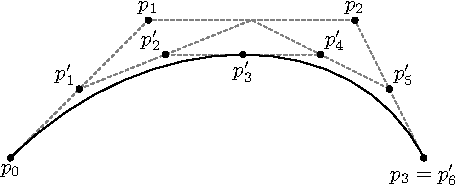
\includegraphics{subdivision}
	     \caption{A Figure}
	 \label{subd}
	\end{figure}

\clearpage %% starts a new page and stops trying to place floats such as tables and figures

\section{More Figure Stuff}
You can also scale and rotate figures.
 	\begin{figure}[h!]
	   
	       \centering
	    % DO NOT ADD A FILENAME EXTENSION TO THE GRAPHIC FILE
	    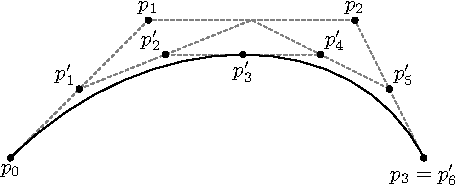
\includegraphics[scale=0.5,angle=180]{subdivision}
	    % if your figure shows up not where you want it, it may just be too big to fit. You can use the scale argument to shrink it, e.g. scale=0.85 is 85 percent of the original size. 
	     \caption{A Smaller Figure, Flipped Upside Down}
	 \label{subd2}
	\end{figure}

\section{Even More Figure Stuff}
With some clever work you can crop a figure, which is handy if (for instance) your EPS or PDF is a little graphic on a whole sheet of paper. The viewport arguments are the lower-left and upper-right coordinates for the area you want to crop.

 	\begin{figure}[h!]
	    	       \centering
	    % DO NOT ADD A FILENAME EXTENSION TO THE GRAPHIC FILE
	   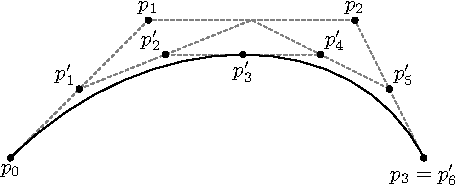
\includegraphics[clip=true, viewport=.0in .0in 1in 1in]{subdivision}
	    \caption{A Cropped Figure}
	 \label{subd3}
	\end{figure}
	
      \subsection{Common Modifications}
      The following figure features the more popular changes thesis students want to their figures. This information is also on the web at \url{web.reed.edu/cis/help/latex/graphics.html}.
           \renewcommand{\thefigure}{0.\arabic{figure}} %Renumbers the figure to the type 0.x
    \addtocounter{figure}{4} %starts the figure numbering at 4
    \begin{figure}[htbp]
    \begin{center}
   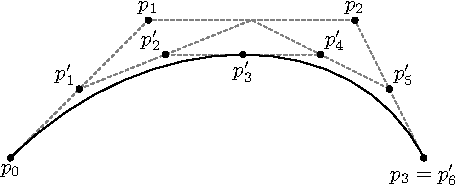
\includegraphics[scale=0.5]{subdivision}
    \caption[Flower type and percent specialization]{\footnotesize{Interaction bar plot showing the degree of specialization for each flower type.}} %the special ToC caption is in square brackets. The \footnotesize makes the figure caption smaller
    \label{barplot}
    \end{center}
    \end{figure} 

	%\chapter*{Conclusion}
         \addcontentsline{toc}{chapter}{Conclusion}
	\chaptermark{Conclusion}
	\markboth{Conclusion}{Conclusion}
	\setcounter{chapter}{4}
	\setcounter{section}{0}
	
Here's a conclusion, demonstrating the use of all that manual incrementing and table of contents adding that has to happen if you use the starred form of the chapter command. The deal is, the chapter command in \LaTeX\ does a lot of things: it increments the chapter counter, it resets the section counter to zero, it puts the name of the chapter into the table of contents and the running headers, and probably some other stuff. 

So, if you remove all that stuff because you don't like it to say ``Chapter 4: Conclusion'', then you have to manually add all the things \LaTeX\ would normally do for you. Maybe someday we'll write a new chapter macro that doesn't add ``Chapter X'' to the beginning of every chapter title.

\section{More info}
And here's some other random info: the first paragraph after a chapter title or section head \emph{shouldn't be} indented, because indents are to tell the reader that you're starting a new paragraph. Since that's obvious after a chapter or section title, proper typesetting doesn't add an indent there. 


%If you feel it necessary to include an appendix, it goes here.
	%\appendix

	%\chapter{The First Appendix}
An appendix full of awesome
	%\chapter{The Second Appendix, for Fun}
An appendix full of win


%This is where endnotes are supposed to go, if you have them.
%I have no idea how endnotes work with LaTeX.

  \backmatter % backmatter makes the index and bibliography appear properly in the t.o.c...

% if you're using bibtex, the next line forces every entry in the bibtex file to be included
% in your bibliography, regardless of whether or not you've cited it in the thesis.
  \nocite{*}

% Rename my bibliography to be called "Works Cited" and not "References" or ``Bibliography''
% \renewcommand{\bibname}{Works Cited}

%    \bibliographystyle{bsts/mla-good} % there are a variety of styles available; 
%  \bibliographystyle{plainnat}
% replace ``plainnat'' with the style of choice. You can refer to files in the bsts or APA 
% subfolder, e.g. 
% \bibliographystyle{bsts/ScienceReedWeb}  % or
\bibliographystyle{ieeetr} 
\bibliography{thesis}
 % Comment the above two lines and uncomment the next line to use biblatex-chicago.
 %\printbibliography[heading=bibintoc]

% Finally, an index would go here... but it is also optional.
\end{document}
